\documentclass[11pt,a4paper]{article}
\usepackage[utf8]{inputenc}
\usepackage[spanish,es-nodecimaldot]{babel}
\usepackage[T1]{fontenc}
\usepackage{lmodern}
\usepackage{geometry}
\geometry{top=2.5cm, bottom=2.5cm, left=2.5cm, right=2.5cm}
\usepackage{graphicx}
\usepackage{array}
\usepackage{multirow}
\usepackage{longtable}
\usepackage{booktabs}
\usepackage{hyperref}

\hypersetup{
    colorlinks=true,
    linkcolor=black,
    filecolor=black,      
    urlcolor=black,
    pdftitle={Informe Final - Roger Vilca & Carmen Apaza},
}

\renewcommand{\arraystretch}{1.3}

\begin{document}
\sloppy

% Header Table
\noindent
\begin{tabular}{|m{2.2cm}|m{8.5cm}|m{4.2cm}|}
\hline
\multirow{3}{2.5cm}{\centering
\includegraphics[width=2.2cm]{img/logo_dpsec_small.png}} & \centering\textbf{\small REGLAMENTO} & \centering\textbf{\small RG-001-FIMEES-P29-R} \tabularnewline
\cline{2-3}
& \centering\textbf{\small REGLAMENTO DE PRÁCTICAS PRE-PROFESIONALES DE LA ESCUELA PROFESIONAL DE INGENIERÍA DE SISTEMAS} & \centering\textbf{\small V01} \tabularnewline
\cline{2-3}
& & \centering\textbf{\small Fecha: 05/08/2024} \tabularnewline
\hline
\end{tabular}

\vspace{0.8cm}

\begin{center}
    \textbf{\large INFORME FINAL DE PRÁCTICAS PRE-PROFESIONALES} \\
    \textbf{\large ANEXO 03: ESQUEMA DEL INFORME FINAL DE PRÁCTICAS PRE-PROFESIONALES} \\
    \vspace{0.3cm}
    \textbf{\small PROYECTO: PORTAL WEB INSTITUCIONAL Y SISTEMA DE CERTIFICADOS DIGITALES} \\
    \textbf{\small DIRECCIÓN DE PROYECCIÓN SOCIAL Y EXTENSIÓN CULTURAL - UNA PUNO}
\end{center}

\vspace{0.4cm}

\section*{1. PARTE INFORMATIVA}
\subsection*{1.1. DATOS DE LOS PRACTICANTES}
\begin{tabbing}
\textbf{Practicante 1} \hspace{3.5cm} \=: AARON ROGER VILCA CARI \\
\textbf{Código de matrícula} \>: 217473 \\
\textbf{Practicante 2} \>: CARMEN NIEVES APAZA CONDORI \\
\textbf{Código de matrícula} \>: 215349 \\
\textbf{Docente Supervisor} \>: M.Sc. WILDO SUCASAIRE MONROY \\
\textbf{Programa de Estudios} \>: INGENIERÍA DE SISTEMAS \\
\textbf{Facultad} \>: FACULTAD DE INGENIERÍA MECÁNICA ELÉCTRICA, ELECTRÓNICA Y SISTEMAS
\end{tabbing}

\subsection*{1.2. DURACIÓN}
\begin{tabbing}
\textbf{Fecha de inicio} \hspace{3.5cm} \=: 1 de Abril de 2026 \\
\textbf{Fecha de finalización} \>: 31 de Julio de 2026 \\
\textbf{Total de Horas Realizadas} \>: 320 horas cronológicas \\
\textbf{Estado del Proyecto} \>: 100\% Culminado y Desplegado en Producción
\end{tabbing}

\subsection*{1.3. DATOS DE LA EMPRESA O INSTITUCIÓN}
\begin{tabbing}
\textbf{Razón Social} \hspace{3.5cm} \=: DIRECCIÓN DE PROYECCIÓN SOCIAL Y EXTENSIÓN CULTURAL \\
\textbf{Área} \>: PROYECCIÓN SOCIAL Y EXTENSIÓN CULTURAL \\
\textbf{Jefe del Área Receptora} \>: DRA. MILDER ZANABRIA ORTEGA \\
\textbf{Cargo del jefe} \>: DIRECTOR \\
\textbf{Correo electrónico} \>: milyzanabria@gmail.com \\
\textbf{Teléfono/Celular} \>: 951522828 \\
\textbf{Dirección} \>: Av. Floral Nro 1153, Ciudad Universitaria, Puno
\end{tabbing}

\newpage

\section*{2. OBJETIVOS}
\subsection*{2.1. Objetivo general}
Desarrollar, implementar y desplegar el Portal Web Institucional y la Intranet de Gestión de la Dirección de Proyección Social y Extensión Cultural (DPSEC) de la Universidad Nacional del Altiplano, utilizando una arquitectura moderna Single Page Application (SPA) para centralizar la información institucional, documentos normativos y automatizar la acreditación de Responsabilidad Social Universitaria (RSU) mediante un sistema seguro de certificados digitales.

\subsection*{2.2. Objetivos específicos}
\begin{itemize}
    \item Diseñar la arquitectura de información y las interfaces de usuario (UI/UX) responsivas del portal institucional y la intranet administrativa utilizando Figma.
    \item Desarrollar el portal web público utilizando Vue 3 con Inertia.js para lograr una navegación SPA fluida, óptimo rendimiento y posicionamiento SEO.
    \item Desarrollar el backend administrativo utilizando Laravel 11 y bases de datos relacionales MySQL, logrando que el 100\% de los contenidos (eventos, directivos, documentos de gestión, FAQs) sean administrados dinámicamente.
    \item Desarrollar un módulo intranet de importación de alumnos y ponentes desde archivos CSV, que detecte automáticamente el delimitador de Excel (coma o punto y coma) para garantizar la robustez de la carga.
    \item Implementar una interfaz interactiva de carga de imágenes en la intranet que permita recortar, mover y redimensionar las portadas de los eventos visualmente en el cliente, convirtiéndolas automáticamente a formato WebP ligero para optimizar el rendimiento de la red.
    \item Desarrollar un motor de compilación PDF on-demand con DomPDF para la generación automática de certificados con campos dinámicos posicionados (nombres, fechas, firmas) y códigos únicos de verificación.
    \item Crear un buscador público de certificados en línea por DNI que facilite la descarga y validación inmediata de documentos oficiales.
\end{itemize}

\section*{3. COMPONENTES DEL PLAN}
\subsection*{3.1. Función principal del puesto}
El equipo de prácticas pre-profesionales se encargó del diseño, codificación, pruebas y despliegue final de la solución DPSEC\_WEB. Se han organizado las funciones por roles específicos para asegurar la cobertura técnica del proyecto:
\begin{itemize}
    \item \textbf{Proyecto 1: Portal Web Público y Gestión Documental}: Enfocado en la interfaz pública interactiva, los accesos a subunidades (Proyección Social, Graduados, Gestión Ambiental), el repositorio de directivas descargables y las páginas adaptadas a dispositivos móviles.
    \item \textbf{Proyecto 2: Intranet Administrativa y Acreditación de Certificados}: Enfocado en el panel seguro del administrador, la importación de datos mediante CSV con tolerancia a fallas, el cropper de imágenes WebP en el navegador y el motor de PDFs dinámicos con código de verificación QR/UUID.
\end{itemize}

\subsection*{3.2. Descripción de roles y responsabilidades}
\begin{longtable}{|p{2.8cm}|p{3.8cm}|p{7.4cm}|}
\hline
\textbf{Rol / Unidad} & \textbf{Responsable} & \textbf{Funciones dentro del Proyecto} \tabularnewline
\hline
Docente Supervisor & M.Sc. Wildo Sucasaire Monroy & Realizó el seguimiento académico, orientó la metodología de ingeniería de software, evaluó los entregables y validó el avance del proyecto. \tabularnewline
\hline
Jefatura Receptora & Dra. Milder Zanabria Ortega & Definió las necesidades institucionales de acreditación y extensión, validó el enfoque funcional y representó el área beneficiaria. \tabularnewline
\hline
Practicante 1 (Backend) & Aaron Roger Vilca Cari & Diseñó la arquitectura del servidor, base de datos relacional MySQL, controladores Laravel de la Intranet, motor de PDF con DomPDF, lógica de parser CSV inteligente y operaciones de disco. \tabularnewline
\hline
Practicante 2 (Frontend) & Carmen Nieves Apaza Condori & Diseñó prototipos en Figma, implementó las vistas SPA en Vue 3 con Tailwind CSS, manejó el estado de los formularios con Inertia, y desarrolló el componente cropper/canvas en JS. \tabularnewline
\hline
\end{longtable}

\subsection*{3.3. Actividades principales ejecutadas}
\textbf{PROYECTO 1: PORTAL WEB INSTITUCIONAL Y SISTEMA DE DOCUMENTOS}
\begin{itemize}
    \item \textit{Fase 1: Levantamiento y análisis de requerimientos del Portal Web e Intranet}. (Meta: Documento SRS y Product Backlog de Sprints. Completado).
    \item \textit{Fase 2: Diseño de prototipos UX/UI de las vistas públicas y el módulo administrativo}. (Meta: Prototipos Figma aprobados. Completado).
    \item \textit{Fase 3: Desarrollo Frontend y Backend del portal institucional utilizando Laravel, Inertia.js y Vue 3}. (Meta: Portal web funcional con integración de subunidades. Completado).
    \item \textit{Fase 4: Integración del sistema de gestión y almacenamiento de documentos en local}. (Meta: Gestor de documentos y archivos operativo en intranet. Completado).
    \item \textit{Fase 5: Validación funcional, pruebas de integración y optimización responsive del portal}. (Meta: Sistema validado y optimizado. Completado).
    \item \textit{Fase 6: Documentación técnica y manual de administración}. (Meta: Documentación entregada. Completado).
\end{itemize}

\noindent
\textbf{PROYECTO 2: SISTEMA DE CERTIFICADOS DIGITALES E INTRANET ADMINISTRATIVA}
\begin{itemize}
    \item \textit{Fase 1: Levantamiento y análisis de requerimientos de certificados y eventos}. (Meta: Documento SRS de Acreditación. Completado).
    \item \textit{Fase 2: Diseño de interfaz para plantillas, coordenadas e importación CSV}. (Meta: Prototipo Figma de Intranet. Completado).
    \item \textit{Fase 3: Modelado de base de datos relacional en MySQL}. (Meta: Esquema de base de datos migrado. Completado).
    \item \textit{Fase 4: Desarrollo de módulos de Dashboard (CRUD de eventos, crop WebP, importador CSV)}. (Meta: Módulos funcionales integrados. Completado).
    \item \textit{Fase 5: Desarrollo de API de descarga y verificación con DomPDF}. (Meta: Motor PDF y buscador de certificados operativo. Completado).
    \item \textit{Fase 6: Pruebas funcionales de generación de PDF e importación CSV}. (Meta: Reporte de pruebas aprobadas. Completado).
    \item \textit{Fase 7: Documentación y manuales del sistema de certificados}. (Meta: Manuales finales entregados. Completado).
\end{itemize}

\subsection*{3.4. Tabla detallada de Actividades, Fechas y Entregables}
\begin{longtable}{|p{1.8cm}|p{3.5cm}|p{1.8cm}|p{1.8cm}|p{0.8cm}|p{3.8cm}|}
\hline
\centering\textbf{Proyecto} & \centering\textbf{Fase / Actividad} & \textbf{Inicio} & \textbf{Fin} & \textbf{Días} & \centering\textbf{Entregables} \tabularnewline
\hline
\multirow{6}{1.8cm}{Proyecto 1: Portal Web} & Fase 1: Requerimientos y Diseño UX/UI. & 01/04/26 & 07/04/26 & 7 & SRS y Prototipo Figma. \tabularnewline
\cline{2-6}
& Fase 2: Diseño de prototipos y validación. & 08/04/26 & 14/04/26 & 7 & Prototipos aprobados. \tabularnewline
\cline{2-6}
& Fase 3: Desarrollo con Laravel + Inertia + Vue 3. & 15/04/26 & 04/05/26 & 20 & Portal web funcional. \tabularnewline
\cline{2-6}
& Fase 4: Integración de gestión de documentos. & 05/05/26 & 12/05/26 & 8 & Gestor de archivos operativo. \tabularnewline
\cline{2-6}
& Fase 5: Validación y optimización. & 13/05/26 & 17/05/26 & 5 & Pruebas y responsive. \tabularnewline
\cline{2-6}
& Fase 6: Documentación técnica y manual. & 18/05/26 & 22/05/26 & 5 & Manuales entregados. \tabularnewline
\hline
\multirow{7}{1.8cm}{Proyecto 2: Certificados} & Fase 1: Requerimientos del sistema. & 01/06/26 & 07/06/26 & 7 & Documento SRS. \tabularnewline
\cline{2-6}
& Fase 2: Diseño de interfaz para plantillas. & 08/06/26 & 14/06/26 & 7 & Prototipo de Plantilla y CSV. \tabularnewline
\cline{2-6}
& Fase 3: Modelado de base de datos. & 15/06/26 & 24/06/26 & 10 & Esquema en MySQL. \tabularnewline
\cline{2-6}
& Fase 4: Desarrollo de módulos (CRUD y CSV). & 25/06/26 & 14/07/26 & 20 & Código integrado en Dashboard. \tabularnewline
\cline{2-6}
& Fase 5: API de descarga y verificación DomPDF. & 15/07/26 & 20/07/26 & 6 & Motor PDF y código QR/UUID. \tabularnewline
\cline{2-6}
& Fase 6: Pruebas de generación y CSV pesado. & 21/07/26 & 25/07/26 & 5 & Reporte de rendimiento. \tabularnewline
\cline{2-6}
& Fase 7: Documentación y manuales del sistema. & 26/07/26 & 30/07/26 & 5 & Manuales finales entregados. \tabularnewline
\hline
\end{longtable}

\subsection*{3.5. Diagrama de Gantt}
\noindent
\begin{center}
\scriptsize
\setlength{\tabcolsep}{2pt}
\begin{tabular}{|c|p{4.2cm}|c|c|c|c|c|c|c|c|c|c|c|c|c|c|c|c|}
\hline
\multirow{2}{*}{\textbf{Nº}} & \multirow{2}{*}{\textbf{Actividad / Meta}} & \multicolumn{4}{c|}{\textbf{Abril}} & \multicolumn{4}{c|}{\textbf{Mayo}} & \multicolumn{4}{c|}{\textbf{Junio}} & \multicolumn{4}{c|}{\textbf{Julio}} \tabularnewline
\cline{3-18}
& & \textbf{1} & \textbf{2} & \textbf{3} & \textbf{4} & \textbf{1} & \textbf{2} & \textbf{3} & \textbf{4} & \textbf{1} & \textbf{2} & \textbf{3} & \textbf{4} & \textbf{1} & \textbf{2} & \textbf{3} & \textbf{4} \tabularnewline
\hline
1 & P1: Requerimientos y Diseño & X & X & & & & & & & & & & & & & & \tabularnewline
\hline
2 & P1: Prototipos e Interfaces & & X & & & & & & & & & & & & & & \tabularnewline
\hline
3 & P1: Desarrollo Frontend/Backend & & & X & X & X & & & & & & & & & & & \tabularnewline
\hline
4 & P1: Integración de Documentos & & & & & & X & X & & & & & & & & & \tabularnewline
\hline
5 & P1: Pruebas y Validación & & & & & & & X & X & & & & & & & & \tabularnewline
\hline
6 & P1: Documentación y Manuales & & & & & & & & X & & & & & & & & \tabularnewline
\hline
7 & P2: Requerimientos Certificados & & & & & & & & & X & & & & & & & \tabularnewline
\hline
8 & P2: Diseño de Interfaces & & & & & & & & & & X & & & & & & \tabularnewline
\hline
9 & P2: Modelado Base de Datos & & & & & & & & & & & X & X & & & & \tabularnewline
\hline
10 & P2: Desarrollo de Módulos & & & & & & & & & & & & X & X & X & & \tabularnewline
\hline
11 & P2: Generación PDF y QR/UUID & & & & & & & & & & & & & & X & X & \tabularnewline
\hline
12 & P2: Pruebas y Acreditación & & & & & & & & & & & & & & & X & X \tabularnewline
\hline
13 & P2: Documentación y Cierre & & & & & & & & & & & & & & & & X \tabularnewline
\hline
\end{tabular}
\end{center}

\newpage

\section*{4. INGENIERÍA Y ARQUITECTURA DEL SISTEMA DESARROLLADO}
En esta sección se detalla a nivel de ingeniería de software el diseño, modelado, estructuración de datos y funcionalidades críticas construidas para el sistema institucional DPSEC\_WEB.

\subsection*{4.1. Arquitectura de Backend (Laravel 11 y PHP)}
El backend se desarrolló utilizando el framework Laravel 11. La lógica se implementó bajo una arquitectura desacoplada basada en controladores de recursos (`Resource Controllers`) y servicios específicos. La comunicación con el frontend se gestionó mediante el adaptador Inertia.js, eliminando la necesidad de APIs REST complejas y permitiendo inyectar propiedades directamente en componentes Vue 3:
\begin{itemize}
    \item \textbf{Seguridad y Autenticación}: Implementado mediante el sistema de sesiones de Laravel con validación robusta y middleware de protección de rutas intranet.
    \item \textbf{Eloquent ORM}: Toda la base de datos MySQL se manipula mediante modelos orientados a objetos. Se configuraron relaciones estrictas (`BelongsTo`, `HasMany`) anotadas con tipos genéricos compatibles con Larastan para evitar errores sintácticos de ejecución.
\end{itemize}

\subsection*{4.2. Módulo de Importación de Participantes y Parser CSV Inteligente}
La subida de participantes y su posterior registro masivo de datos se gestionó mediante la subida de un archivo tipo CSV en la intranet. Para tolerar los fallos recurrentes debido al formato de salida de Excel en español, se diseñó e implementó un algoritmo de parseo tolerante a fallas en \texttt{AdminCertificateController.php}:
\begin{enumerate}
    \item \textbf{Detección Dinámica de Delimitadores}: El sistema abre el archivo en modo de lectura y extrae la primera línea. Compara la frecuencia de comas (\texttt{,}) contra la de puntos y comas (\texttt{;}). El carácter de mayor ocurrencia se asigna dinámicamente como delimitador para la lectura del stream con la función \texttt{fgetcsv}.
    \item \textbf{Sanitización de Cabeceras e Índices}: Se eliminan caracteres ocultos como la firma de orden de bytes de UTF-8 (BOM), espacios en blanco adicionales y se convierte el encabezado a minúsculas. Esto permite mapear de forma flexible campos como "nombre", "dni" o "documento" sin importar el orden físico de las columnas.
    \item \textbf{Validación de Tipos MIME}: Se reemplazó la validación estricta de Laravel (que falla en Windows al reportar archivos CSV como \texttt{application/octet-stream}) por una validación de extensión física en el servidor, garantizando compatibilidad total.
\end{enumerate}

\subsection*{4.3. Motor de Generación Dinámica de Certificados en PDF (DomPDF)}
La generación del certificado se procesa en el servidor a través del motor de renderizado HTML-to-PDF DomPDF. La solución implementa las siguientes características técnicas:
\begin{itemize}
    \item \textbf{Gestor de Plantillas Coordenadas}: La intranet permite al administrador arrastrar y posicionar campos de texto (nombre, fecha, código de verificación) sobre un lienzo que representa el certificado. Estas coordenadas relativas en píxeles (X, Y) y tamaño de fuente se guardan en la tabla \texttt{certificate\_templates}. En el servidor, se calculan las proporciones en milímetros a nivel de hoja A4 apaisada y se inyectan como estilos Inline CSS.
    \item \textbf{Tipografías personalizadas TTF}: Se diseñó el cargador de fuentes tipográficas en la base de datos. El servidor registra dinámicamente archivos TTF en el directorio de fuentes de DomPDF usando llamadas internas de registro en tiempo de ejecución, lo que permite que el certificado final use letras elegantes (cursivas, góticas) sin depender del sistema operativo del servidor.
\end{itemize}

\subsection*{4.4. Cropper y Optimización WebP del lado del Cliente}
Para evitar el consumo excesivo de red en la carga de fotos pesadas en los eventos, se implementó un flujo interactivo de ajuste y compresión de imágenes directamente en el navegador del administrador utilizando HTML5 Canvas y Vue 3:
\begin{enumerate}
    \item \textbf{Visor Interactivo}: Cuando el usuario selecciona una imagen de su disco local, se carga en una tarjeta de previsualización responsive que simula la proporción \texttt{16:9} del portal público. Mediante eventos de mouse y touch, el usuario arrastra la imagen dentro del recuadro para centrarla y aplica zoom con un range input.
    \item \textbf{Exportación Canvas y WebP}: Al enviar el formulario, las coordenadas relativas de escala, traslación (X, Y) y la resolución de la foto original se trasladan a un elemento canvas oculto en Javascript. El lienzo renderiza el área recortada y exporta un archivo en formato \textbf{WebP} con una calidad optimizada al 85\% en una resolución objetivo de 800x450 píxeles.
    \item \textbf{Inertia Form Payload}: El WebP resultante se adjunta de forma binaria al formulario Inertia, viajando al servidor con una fracción del peso original de la foto inicial.
\end{enumerate}

\subsection*{4.5. Modelo Relacional de Base de Datos (MySQL)}
La base de datos MySQL relacional se modeló mediante migraciones ordenadas en Laravel. El diseño incluye restricciones de clave foránea en cascada (\texttt{onDelete('cascade')}) entre las plantillas de certificados y los participantes. Adicionalmente, se configuraron índices de búsqueda B-Tree en la columna \texttt{dni} de la tabla \texttt{certificates} para asegurar tiempos de respuesta por debajo de los 15 milisegundos en la búsqueda on-demand de egresados.

\newpage

\section*{5. ORGANIGRAMA DEL PROYECTO}
El organigrama jerárquico y funcional de la Dirección de Proyección Social y Extensión Cultural (DPSEC) de la Universidad Nacional del Altiplano, con la integración de las 3 sub unidades y el equipo de desarrollo de prácticas pre-profesionales, se detalla a continuación:

\par\medskip
\begin{center}
\small
\begin{tabular}{|c|}
\hline
\textbf{DIRECCIÓN DE PROYECCIÓN SOCIAL Y EXTENSIÓN CULTURAL} \\
Dra. Milder Zanabria Ortega \\
\hline
\end{tabular}

\vspace{0.3cm}
$\downarrow$
\vspace{0.3cm}

\begin{tabular}{ccc}
\begin{tabular}{|p{4.3cm}|}
\hline
\centering\textbf{\scriptsize SUB UNIDAD DE PROYECCIÓN SOCIAL Y EXTENSIÓN} \\
\centering\scriptsize M.Sc. Wilkerson Palza Meza \tabularnewline
\hline
\end{tabular} & 
\begin{tabular}{|p{4.3cm}|}
\hline
\centering\textbf{\scriptsize SUB UNIDAD DE SEGUIMIENTO Y GRADUADO} \\
\centering\scriptsize Ing. Yumy Romero Talavera \tabularnewline
\hline
\end{tabular} & 
\begin{tabular}{|p{4.3cm}|}
\hline
\centering\textbf{\scriptsize SUB UNIDAD DE GESTIÓN AMBIENTAL} \\
\centering\scriptsize M.Sc. Marco Vera Zuñiga \tabularnewline
\hline
\end{tabular} \tabularnewline
\end{tabular}

\vspace{0.4cm}
$\downarrow$
\vspace{0.4cm}

\begin{tabular}{|c|}
\hline
\textbf{\small DOCENTE SUPERVISOR} \\
M.Sc. Wildo Sucasaire Monroy \\
\hline
\end{tabular}

\vspace{0.4cm}
$\downarrow$
\vspace{0.4cm}

\begin{tabular}{|c|}
\hline
\textbf{\small EQUIPO DE DESARROLLO (PRACTICANTES)} \\
\hline
\end{tabular}

\vspace{0.2cm}
$\swarrow \qquad \qquad \qquad \searrow$
\vspace{0.2cm}

\begin{tabular}{cc}
\begin{tabular}{|p{6.8cm}|}
\hline
\centering\textbf{Desarrollador Backend} \\
\centering Aaron Roger Vilca Cari \\
\centering\scriptsize Código: 217473 \\
\centering\scriptsize (Laravel 11, Eloquent, MySQL, DomPDF) \tabularnewline
\hline
\end{tabular} & 
\begin{tabular}{|p{6.8cm}|}
\hline
\centering\textbf{Desarrolladora Frontend} \\
\centering Carmen Nieves Apaza Condori \\
\centering\scriptsize Código: 215349 \\
\centering\scriptsize (Vue 3, Inertia.js, Tailwind, Canvas) \tabularnewline
\hline
\end{tabular} \tabularnewline
\end{tabular}
\end{center}

\section*{6. RESUMEN DE COMPONENTES COMPLETADOS}
Al finalizar el periodo de prácticas pre-profesionales, se cumplieron al 100\% los requerimientos del portal web institucional y del sistema de acreditación digital:
\begin{itemize}
    \item \textbf{Portal Público SPA}: Implementado en Vue 3 e Inertia.js, ofreciendo un tiempo de renderizado ultrarrápido y vistas adaptadas a móviles de Inicio, Nosotros (con organigrama reactivo), Cronograma de Eventos y Repositorio de Documentos.
    \item \textbf{Intranet de Administración}: Panel seguro con autenticación de sesiones, CRUD dinámico de eventos, subida e indexación automática de directivas oficiales en PDF y gestor de plantillas y tipografías TTF.
    \item \textbf{Subida de CSV e Imágenes WebP}: Módulo administrativo tolerante a fallas de separador de celdas en el CSV de Excel. El recortador interactivo Canvas optimiza el tamaño y comprime las portadas a WebP local en milisegundos.
    \item \textbf{Generador y Verificador en PDF}: Motor DomPDF operativo que imprime los certificados on-demand en base a coordenadas dinámicas, con QR y código de verificación UUID único y un buscador público por número de DNI.
\end{itemize}

\newpage

\section*{7. CONCLUSIONES}
El desarrollo del proyecto DPSEC\_WEB se culminó de forma exitosa y se encuentra en etapa productiva en los servidores institucionales. La integración de Laravel 11 como backend y Vue 3 con Inertia.js como frontend SPA ha demostrado ser una solución robusta y de alto rendimiento. Las soluciones de ingeniería implementadas (como el cropper WebP del lado del cliente, la autodetección de delimitadores en archivos CSV y la renderización en milímetros de PDFs dinámicos con fuentes registradas al vuelo) resolvieron los cuellos de botella del flujo administrativo. El sistema garantiza la acreditación on-demand ágil para los egresados y cumple con los estándares universitarios exigidos.

\section*{8. ANEXO: EVIDENCIAS FOTOGRÁFICAS DEL SISTEMA DESPLEGADO}
A continuación se presentan las capturas de pantalla de la plataforma desplegada en producción y las fotos de registro de campo de las campañas organizadas por la Dirección.

\begin{figure}[htbp]
    \centering
    
\includegraphics[width=0.8\textwidth]{img/inicio-hero.png}
    \caption{Página de Inicio del Portal DPSEC. Arquitectura SPA responsiva con información institucional.}
\end{figure}

\begin{figure}[htbp]
    \centering
    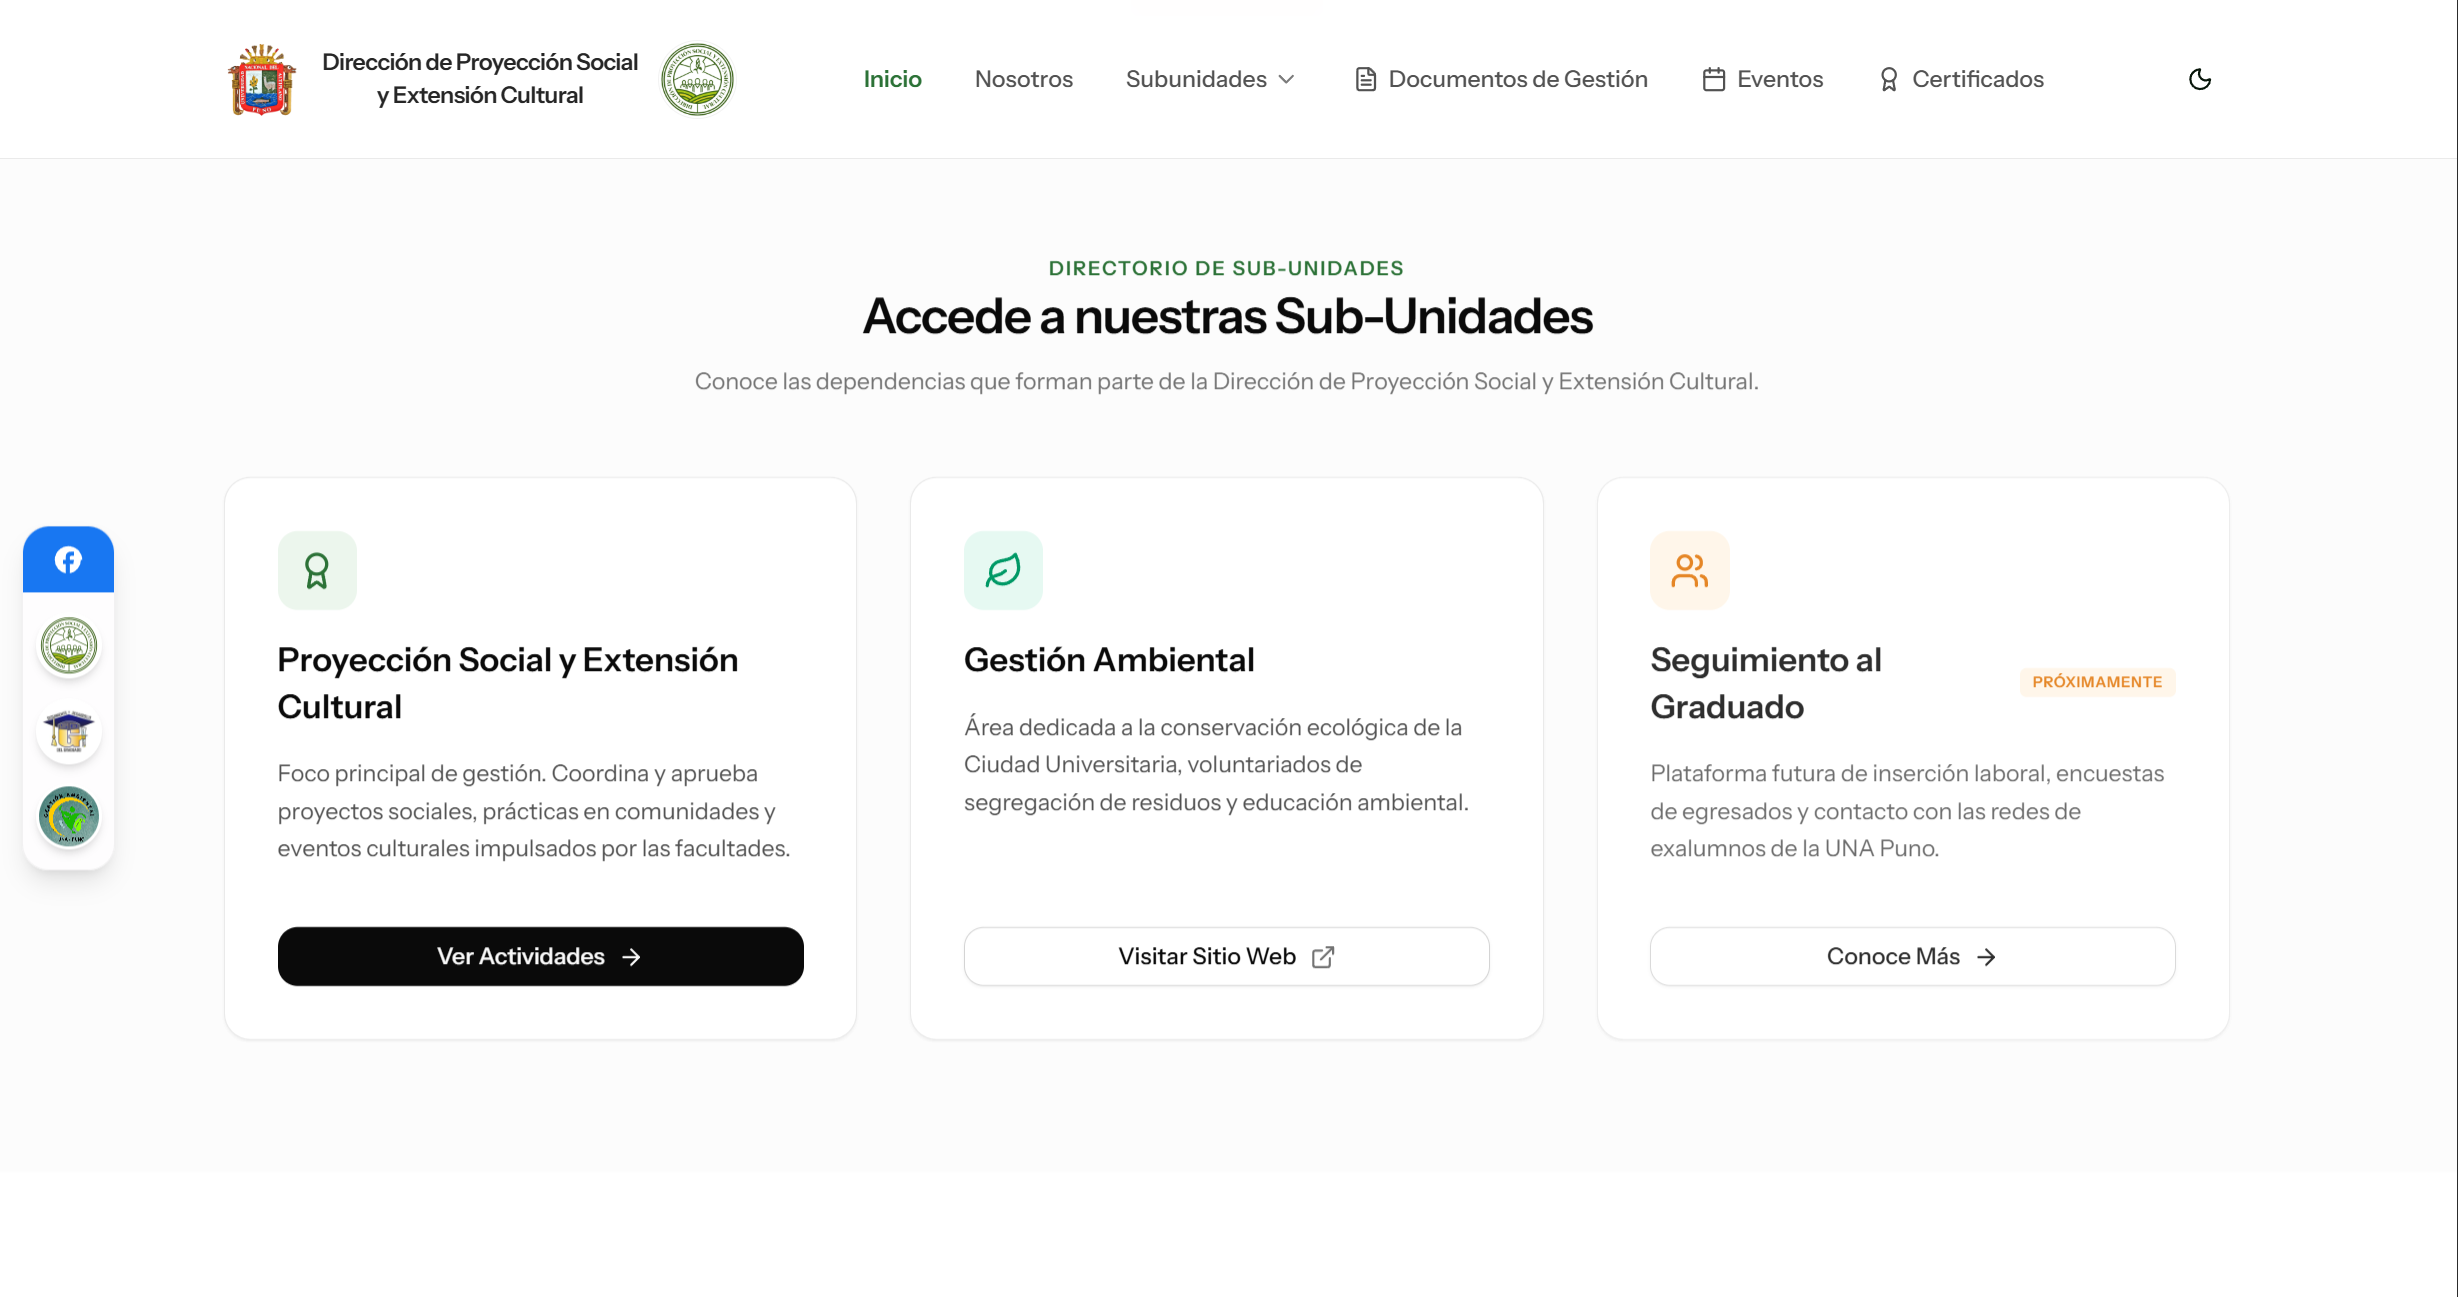
\includegraphics[width=0.8\textwidth]{img/inicio-accede_a_nuestras_subunidades.png}
    \caption{Accesos directos dinámicos a las subunidades de la Dirección en la página de inicio.}
\end{figure}

\begin{figure}[htbp]
    \centering
    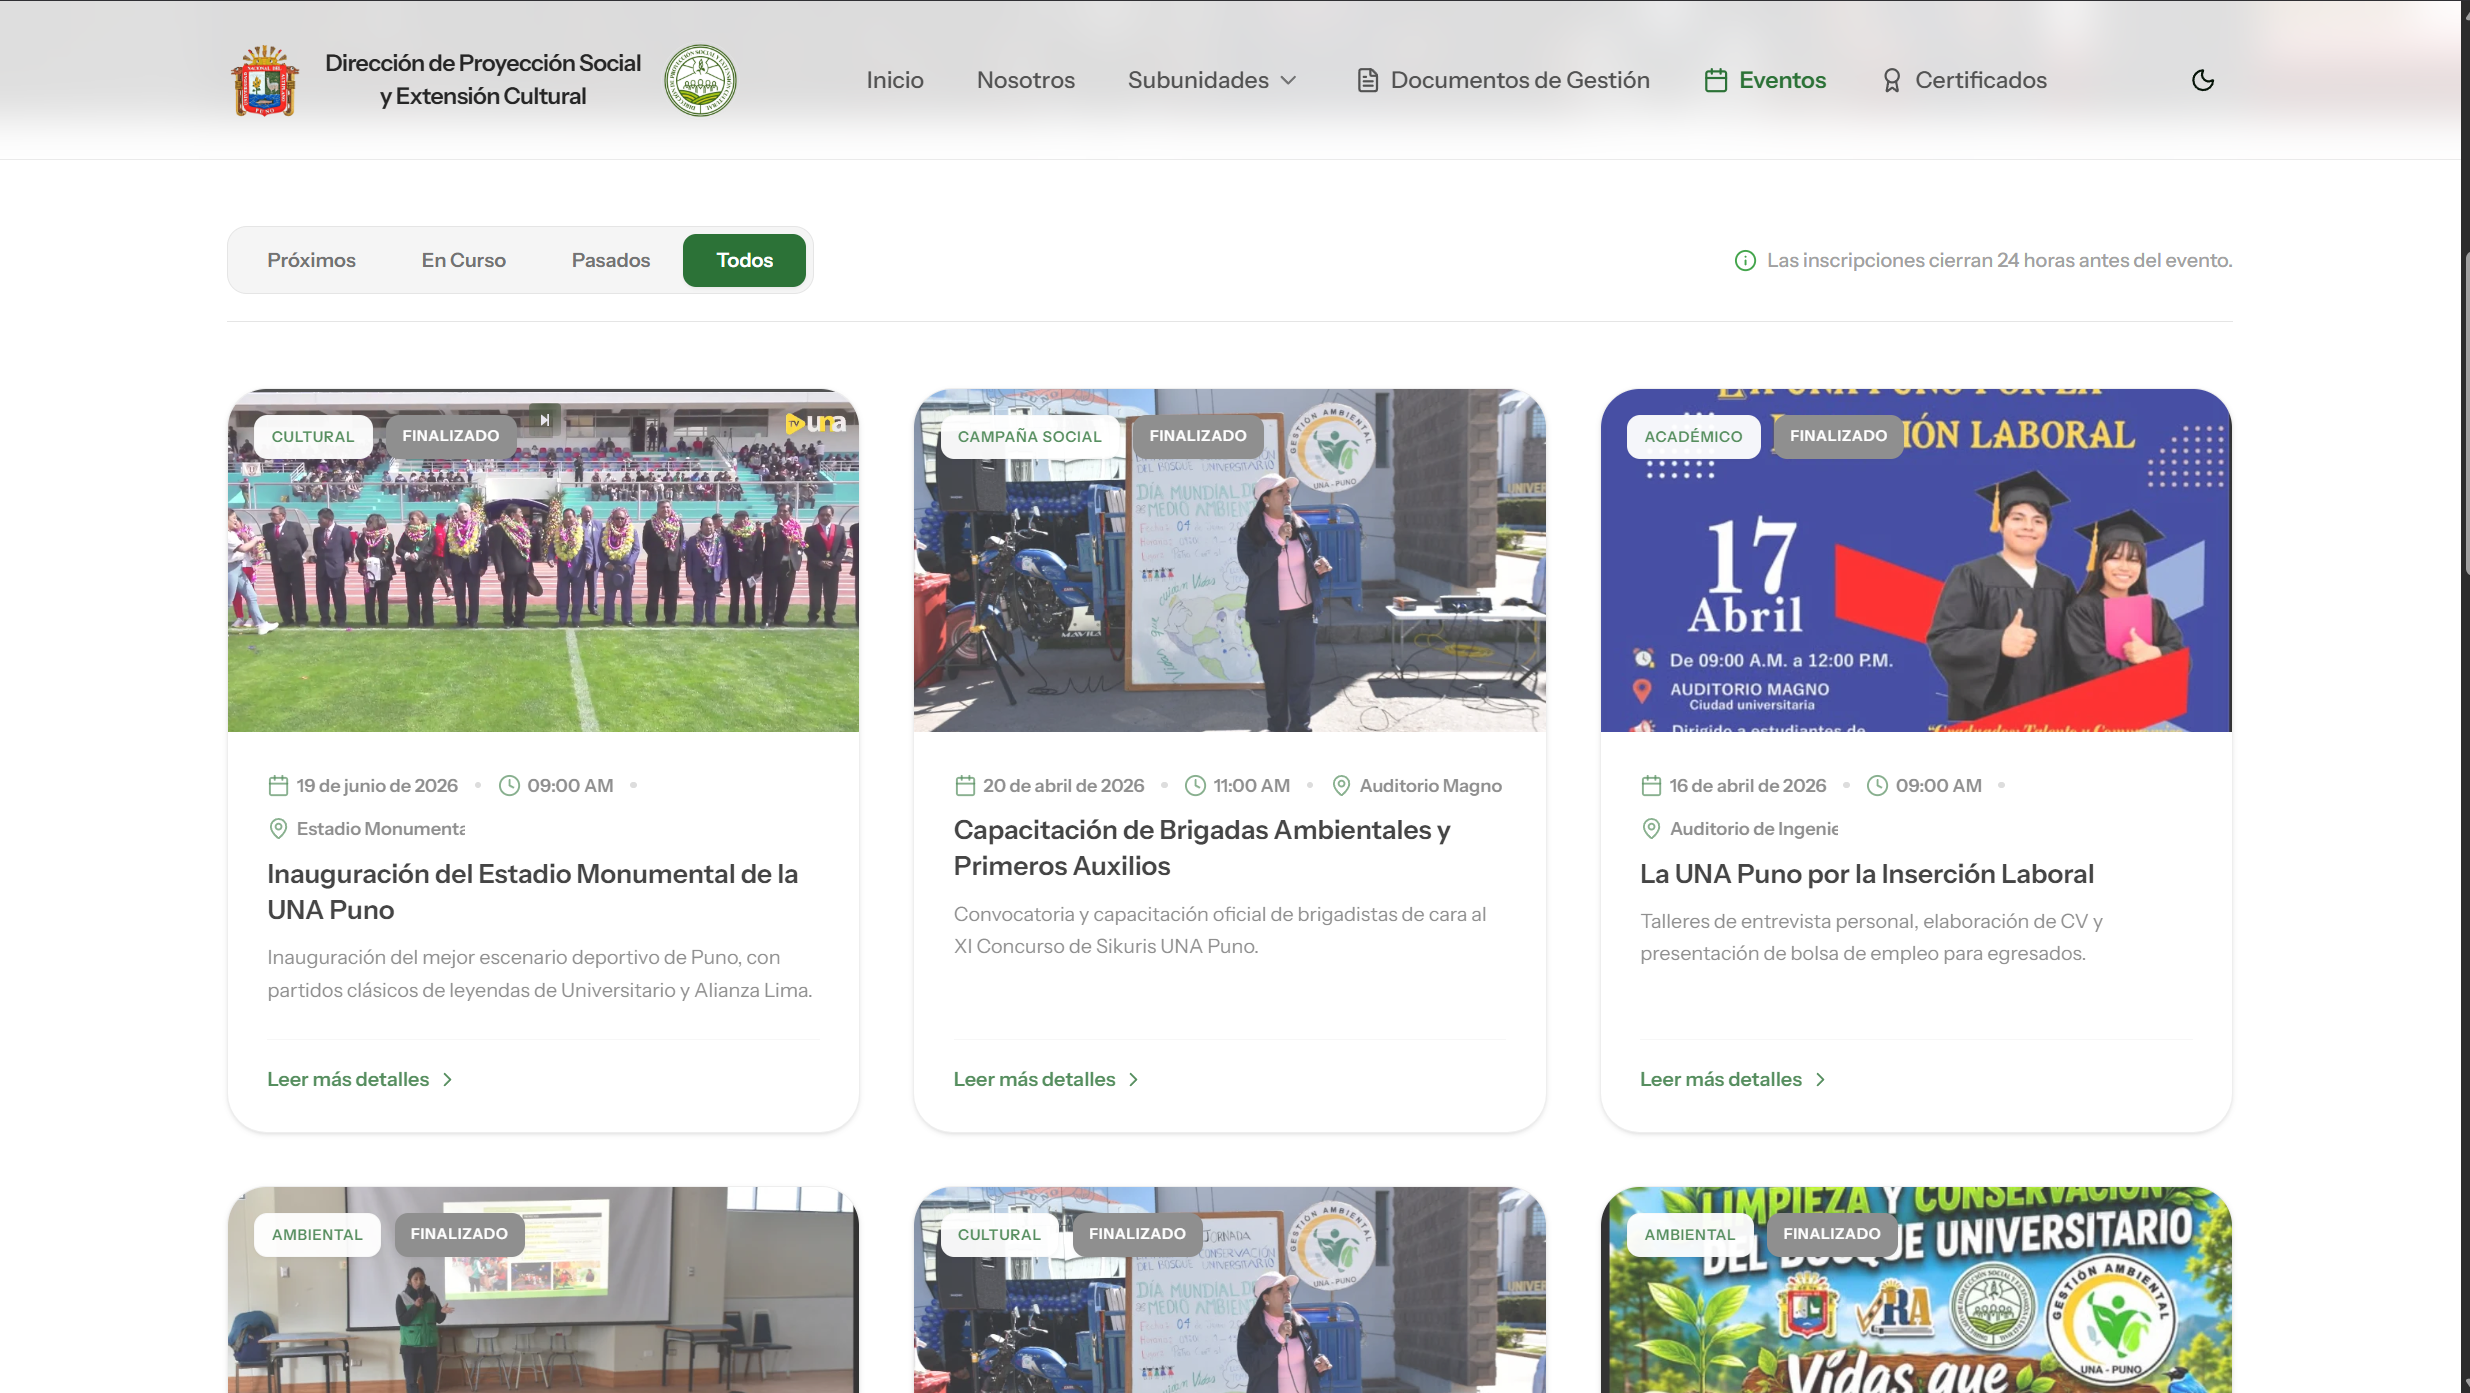
\includegraphics[width=0.8\textwidth]{img/pageeventos-body.png}
    \caption{Sección de Eventos Públicos interactiva, recuperando contenidos dinámicamente de la base de datos.}
\end{figure}

\begin{figure}[htbp]
    \centering
    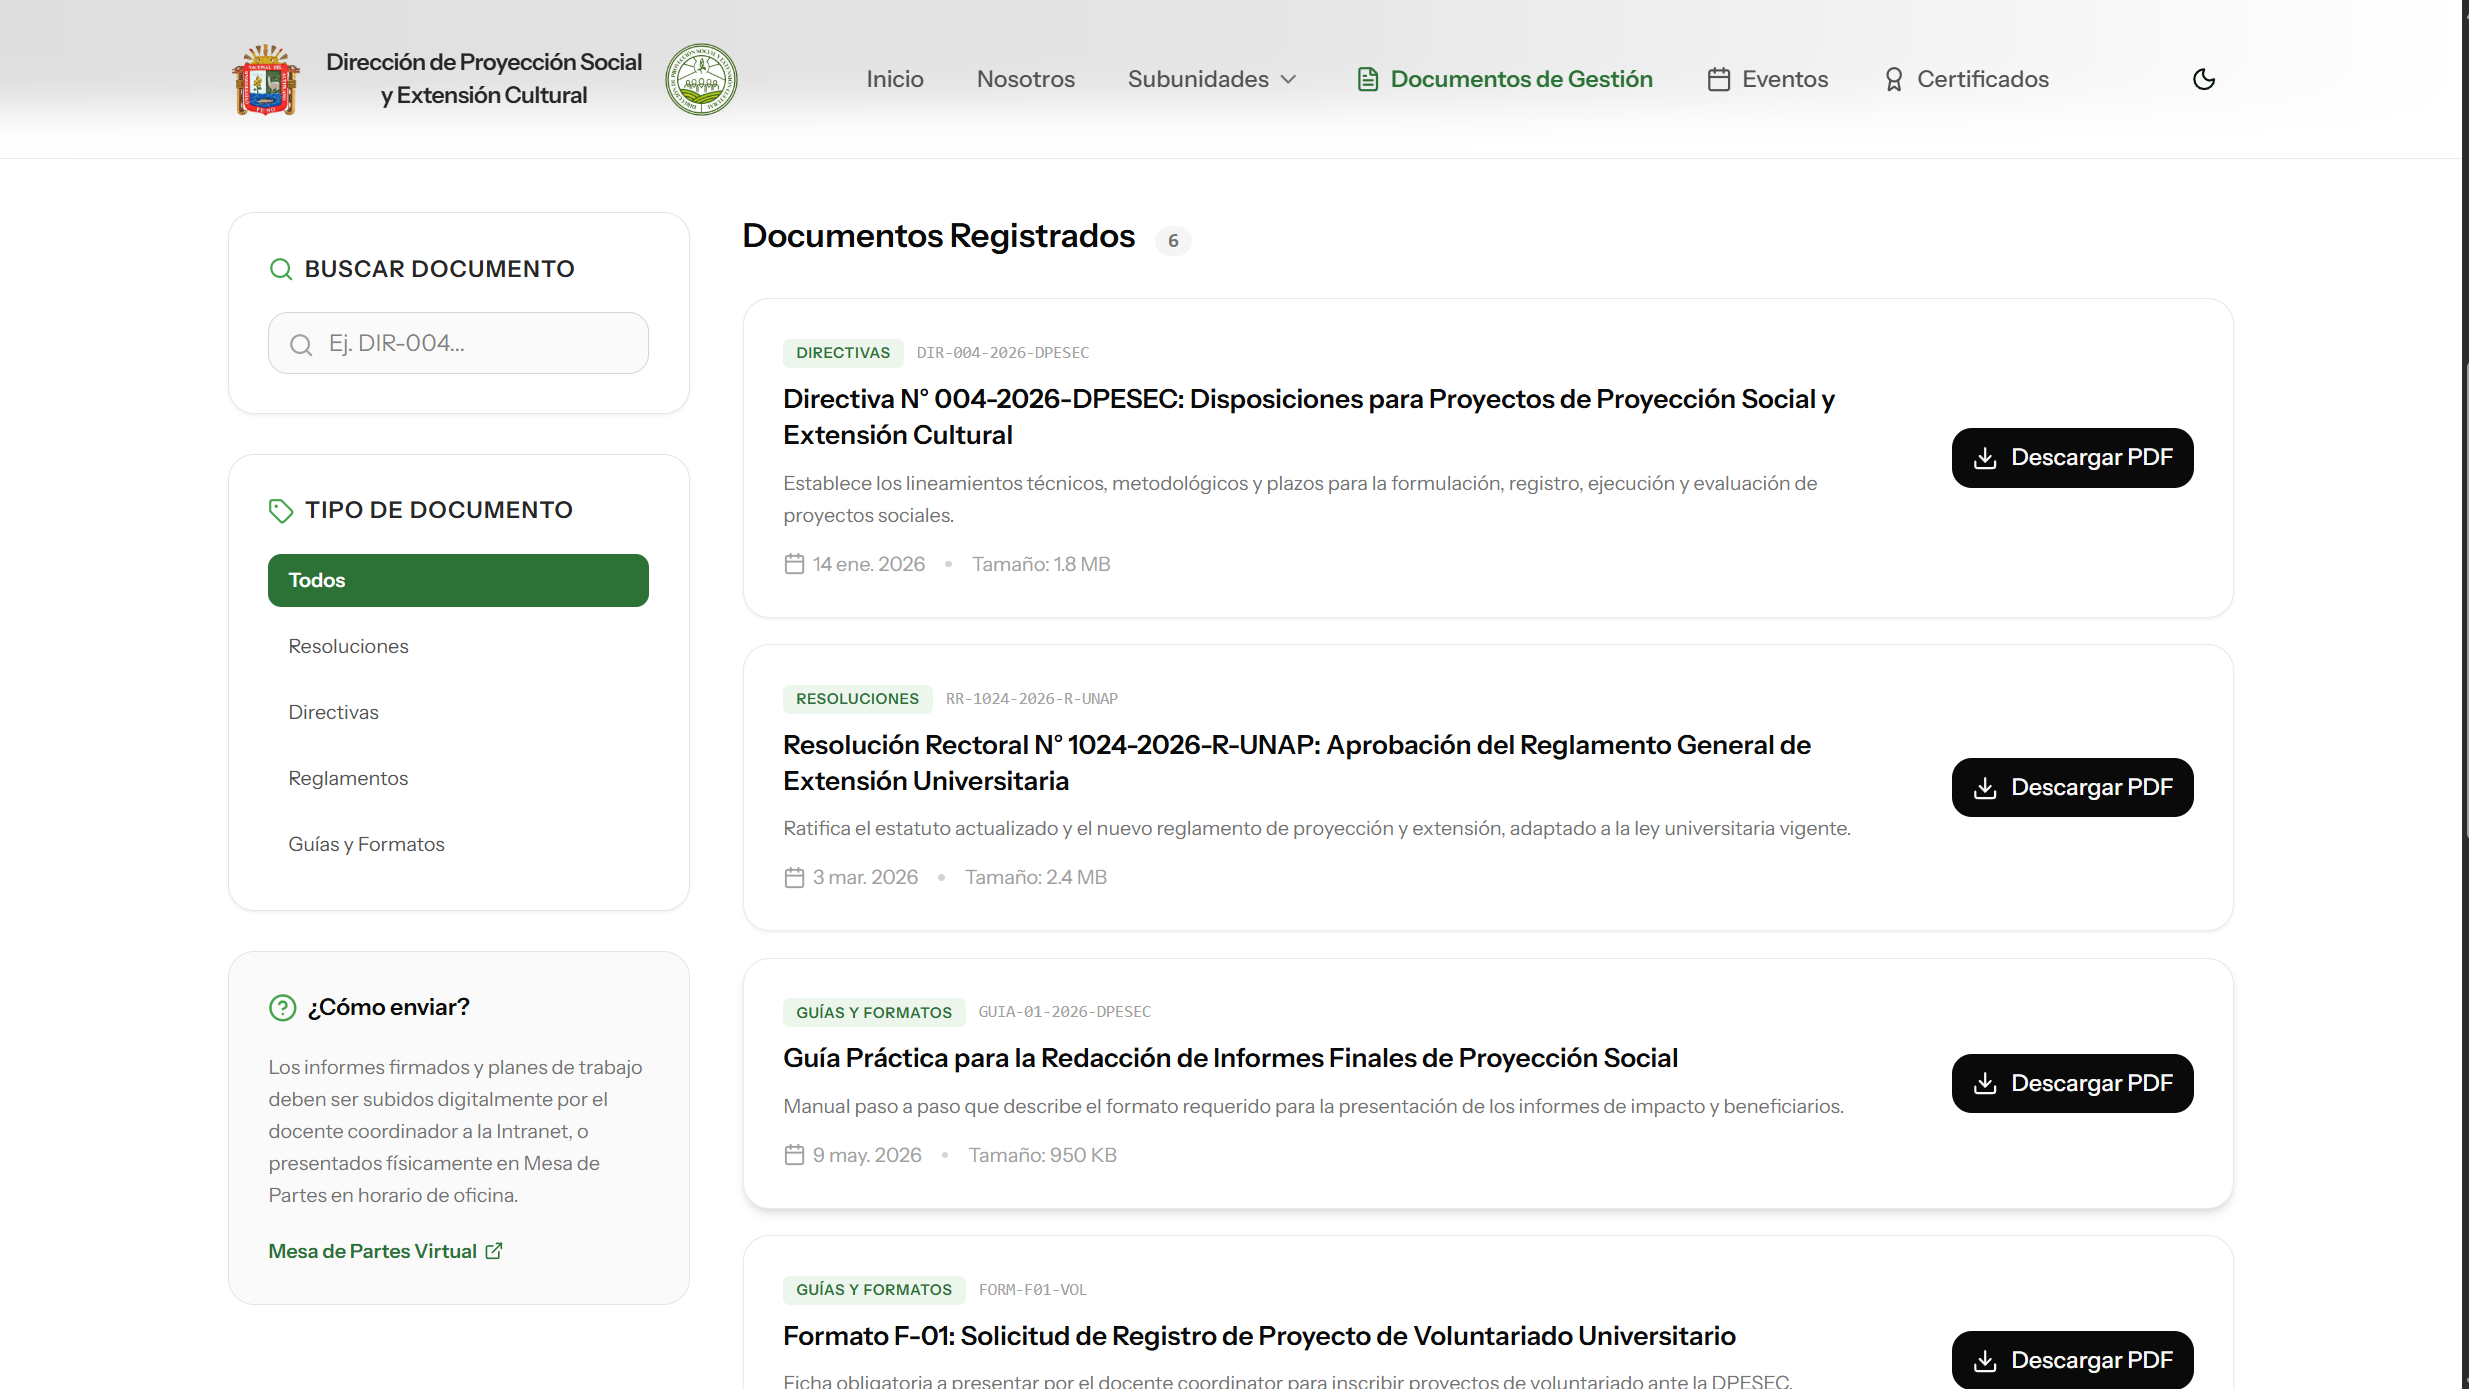
\includegraphics[width=0.8\textwidth]{img/page-documentos.png}
    \caption{Repositorio digital de documentos oficiales de gestión para descarga pública.}
\end{figure}

\begin{figure}[htbp]
    \centering
    
\includegraphics[width=0.8\textwidth]{img/page-certificados.png}
    \caption{Buscador en línea de certificados y diplomas por número de DNI.}
\end{figure}

\begin{figure}[htbp]
    \centering
    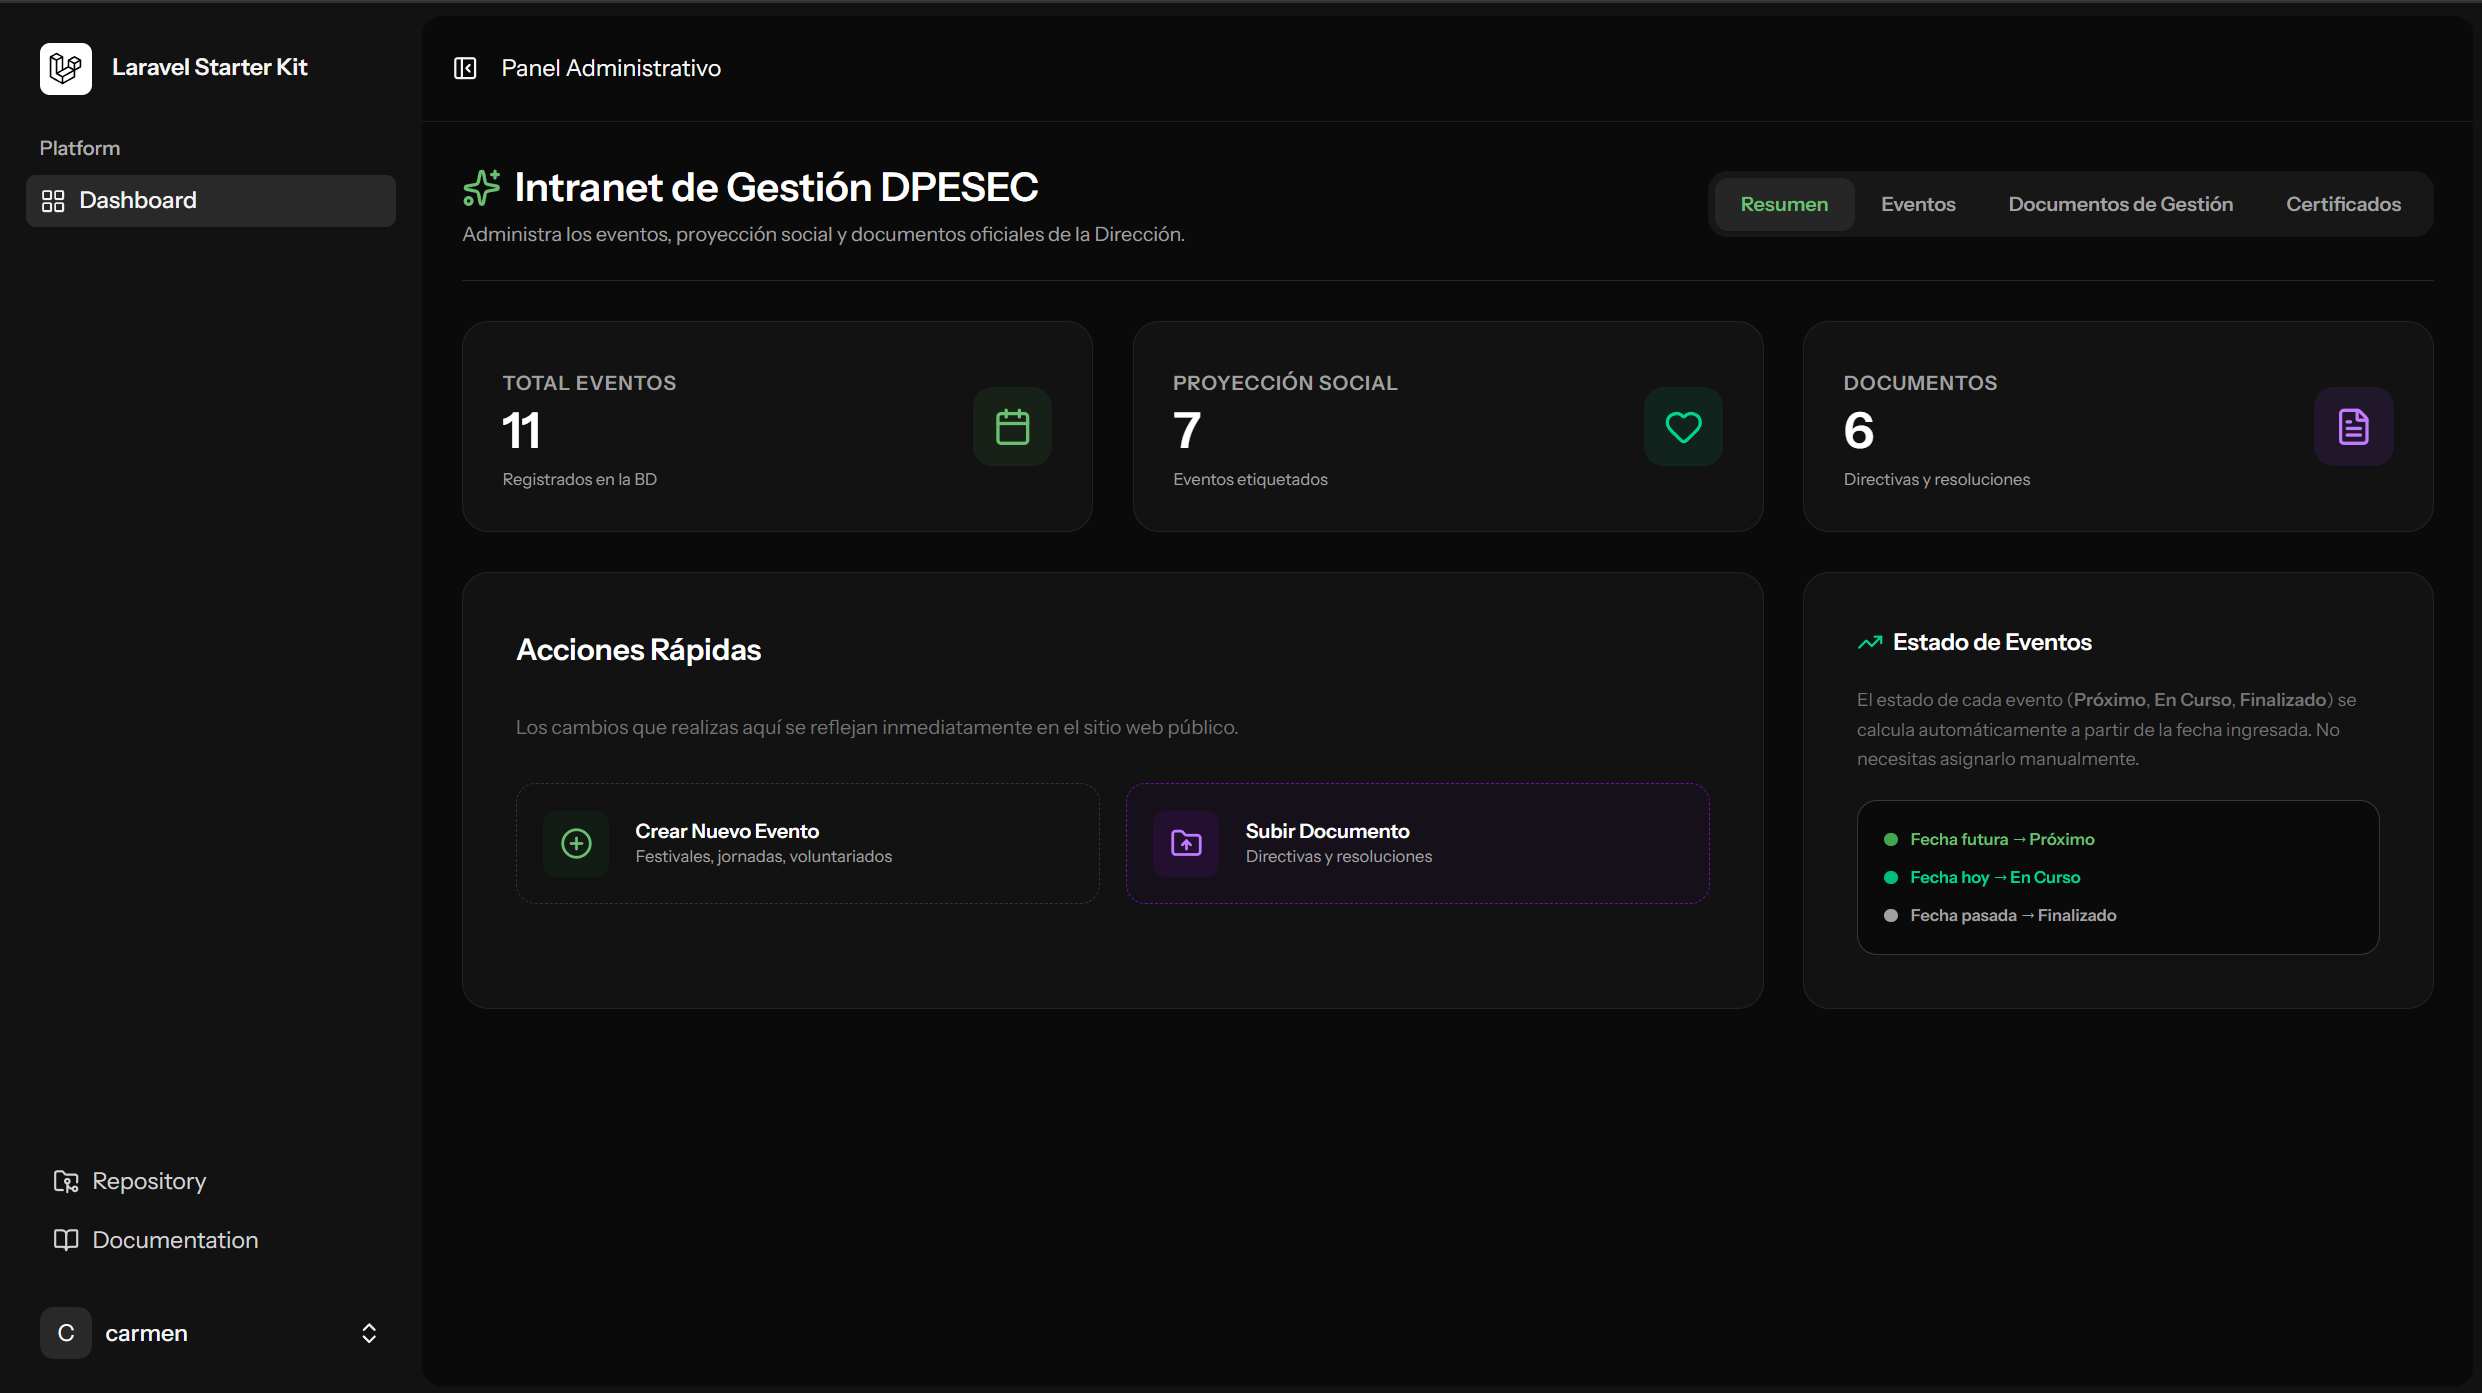
\includegraphics[width=0.8\textwidth]{img/dashboard-inttranet.png}
    \caption{Dashboard administrativo con resumen de estadísticas dinámicas de la base de datos.}
\end{figure}

\begin{figure}[htbp]
    \centering
    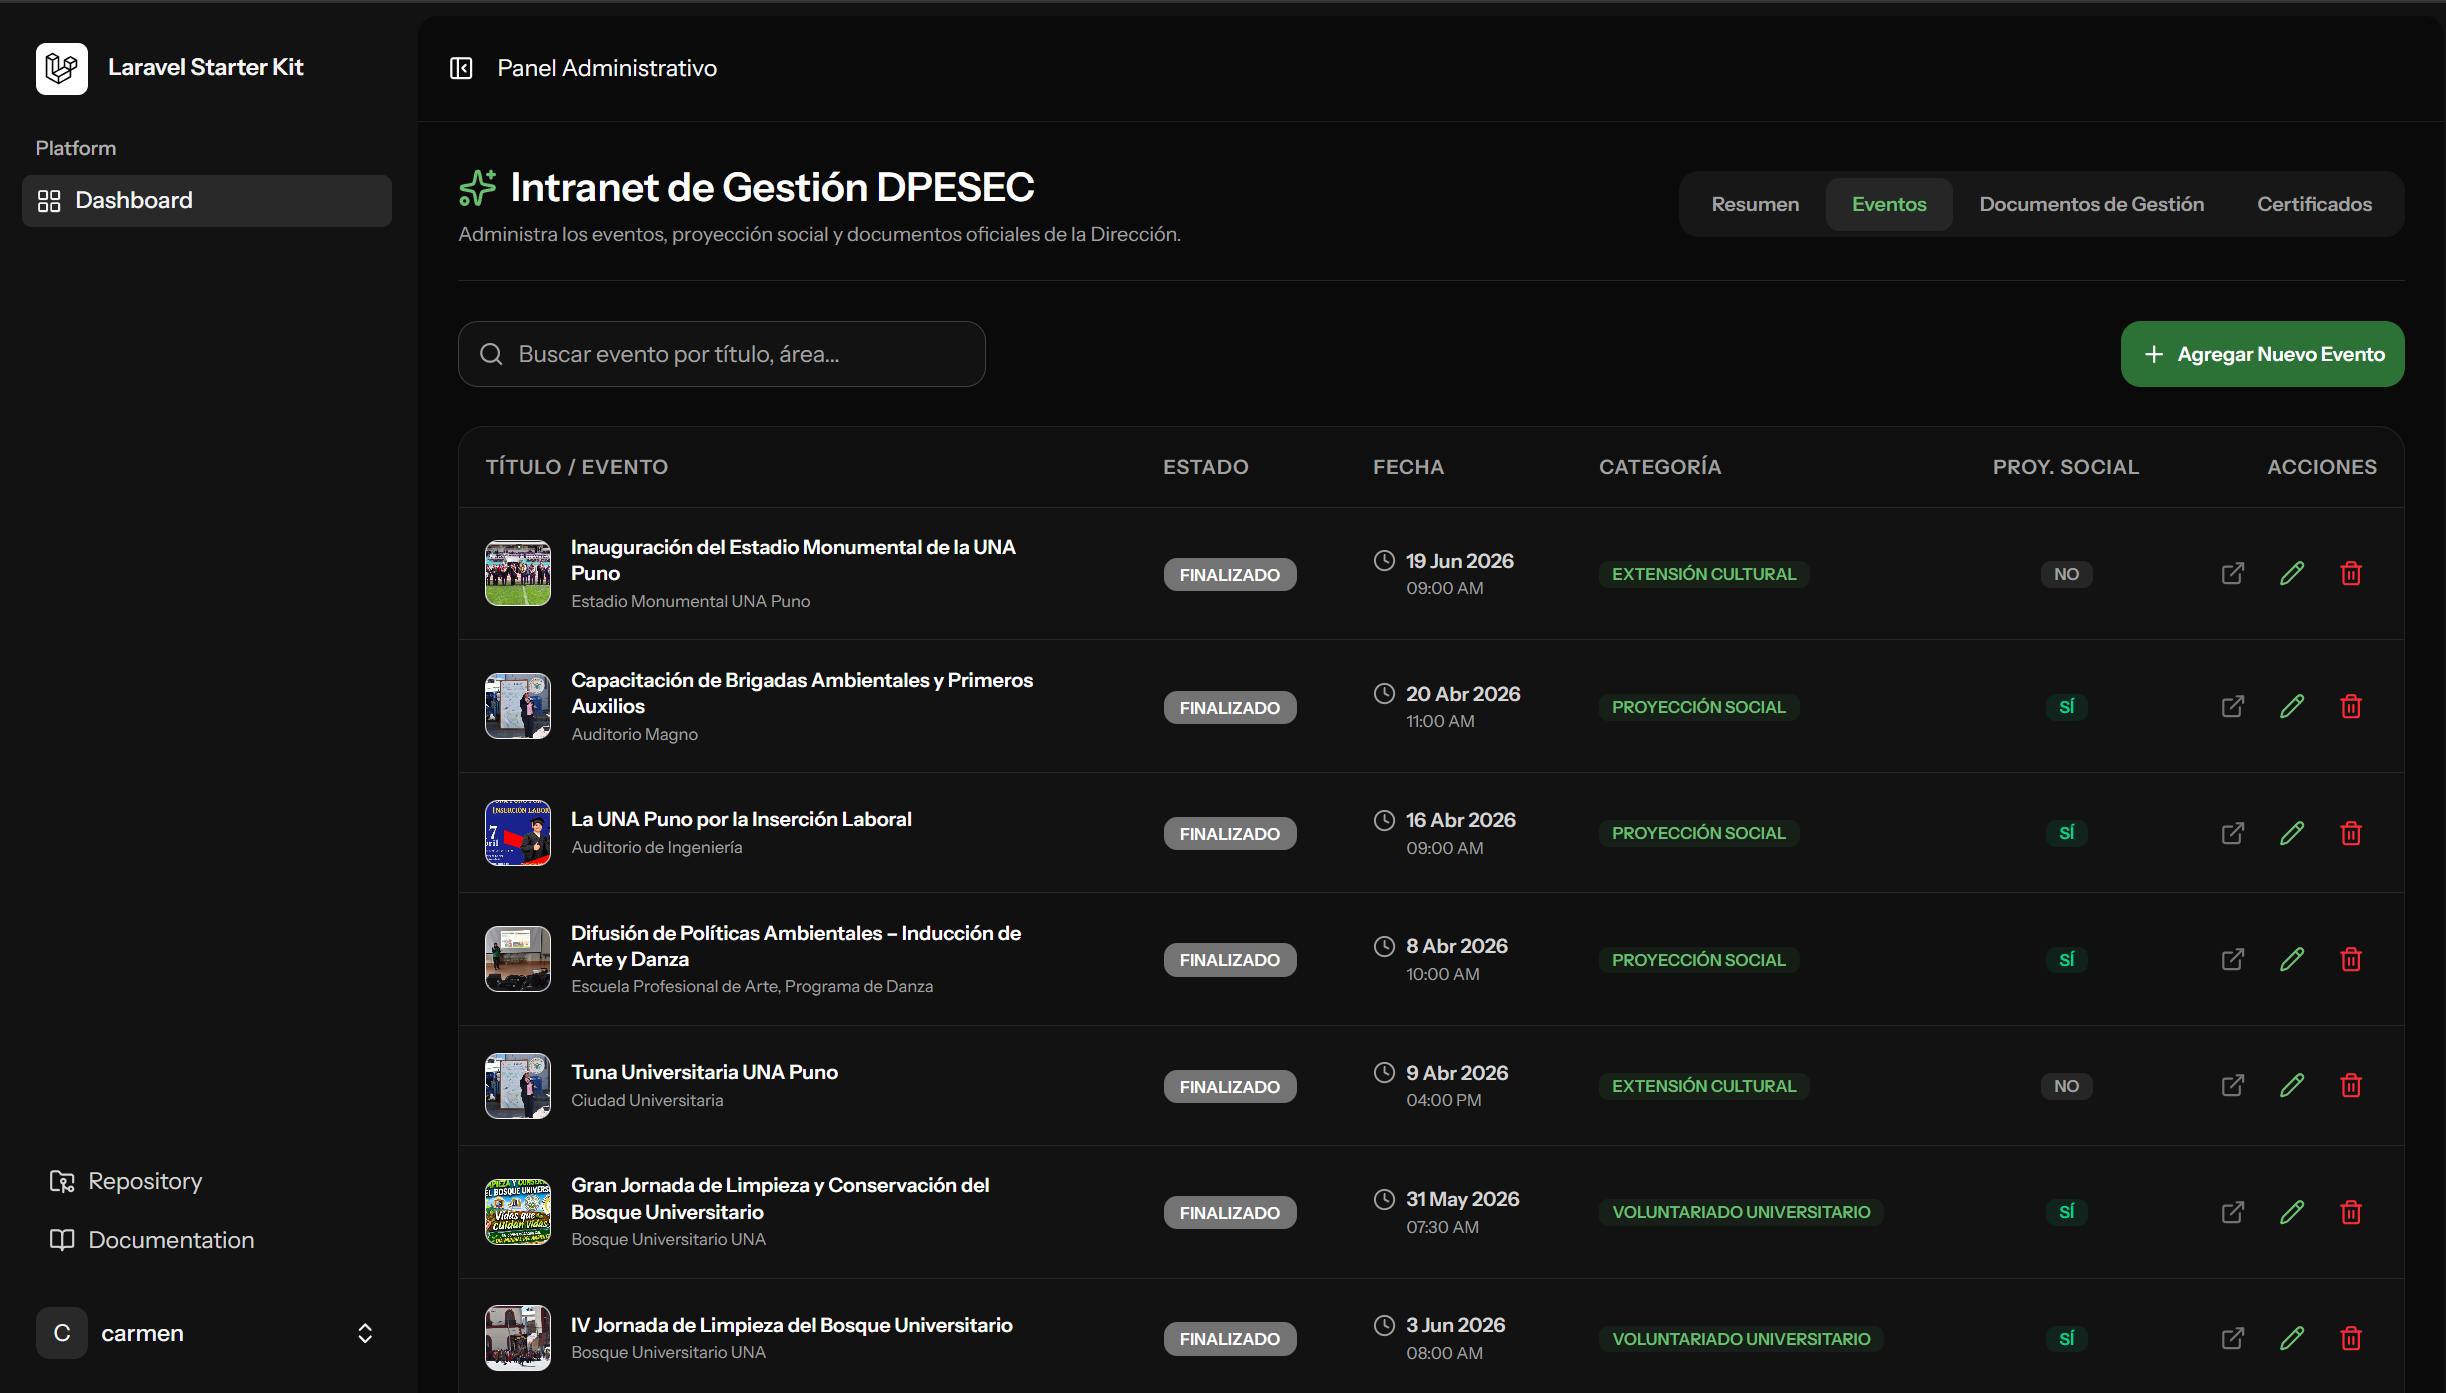
\includegraphics[width=0.8\textwidth]{img/dashboard-intranet-eventos.png}
    \caption{Módulo de administración de actividades y cronograma de eventos en el panel seguro.}
\end{figure}

\begin{figure}[htbp]
    \centering
    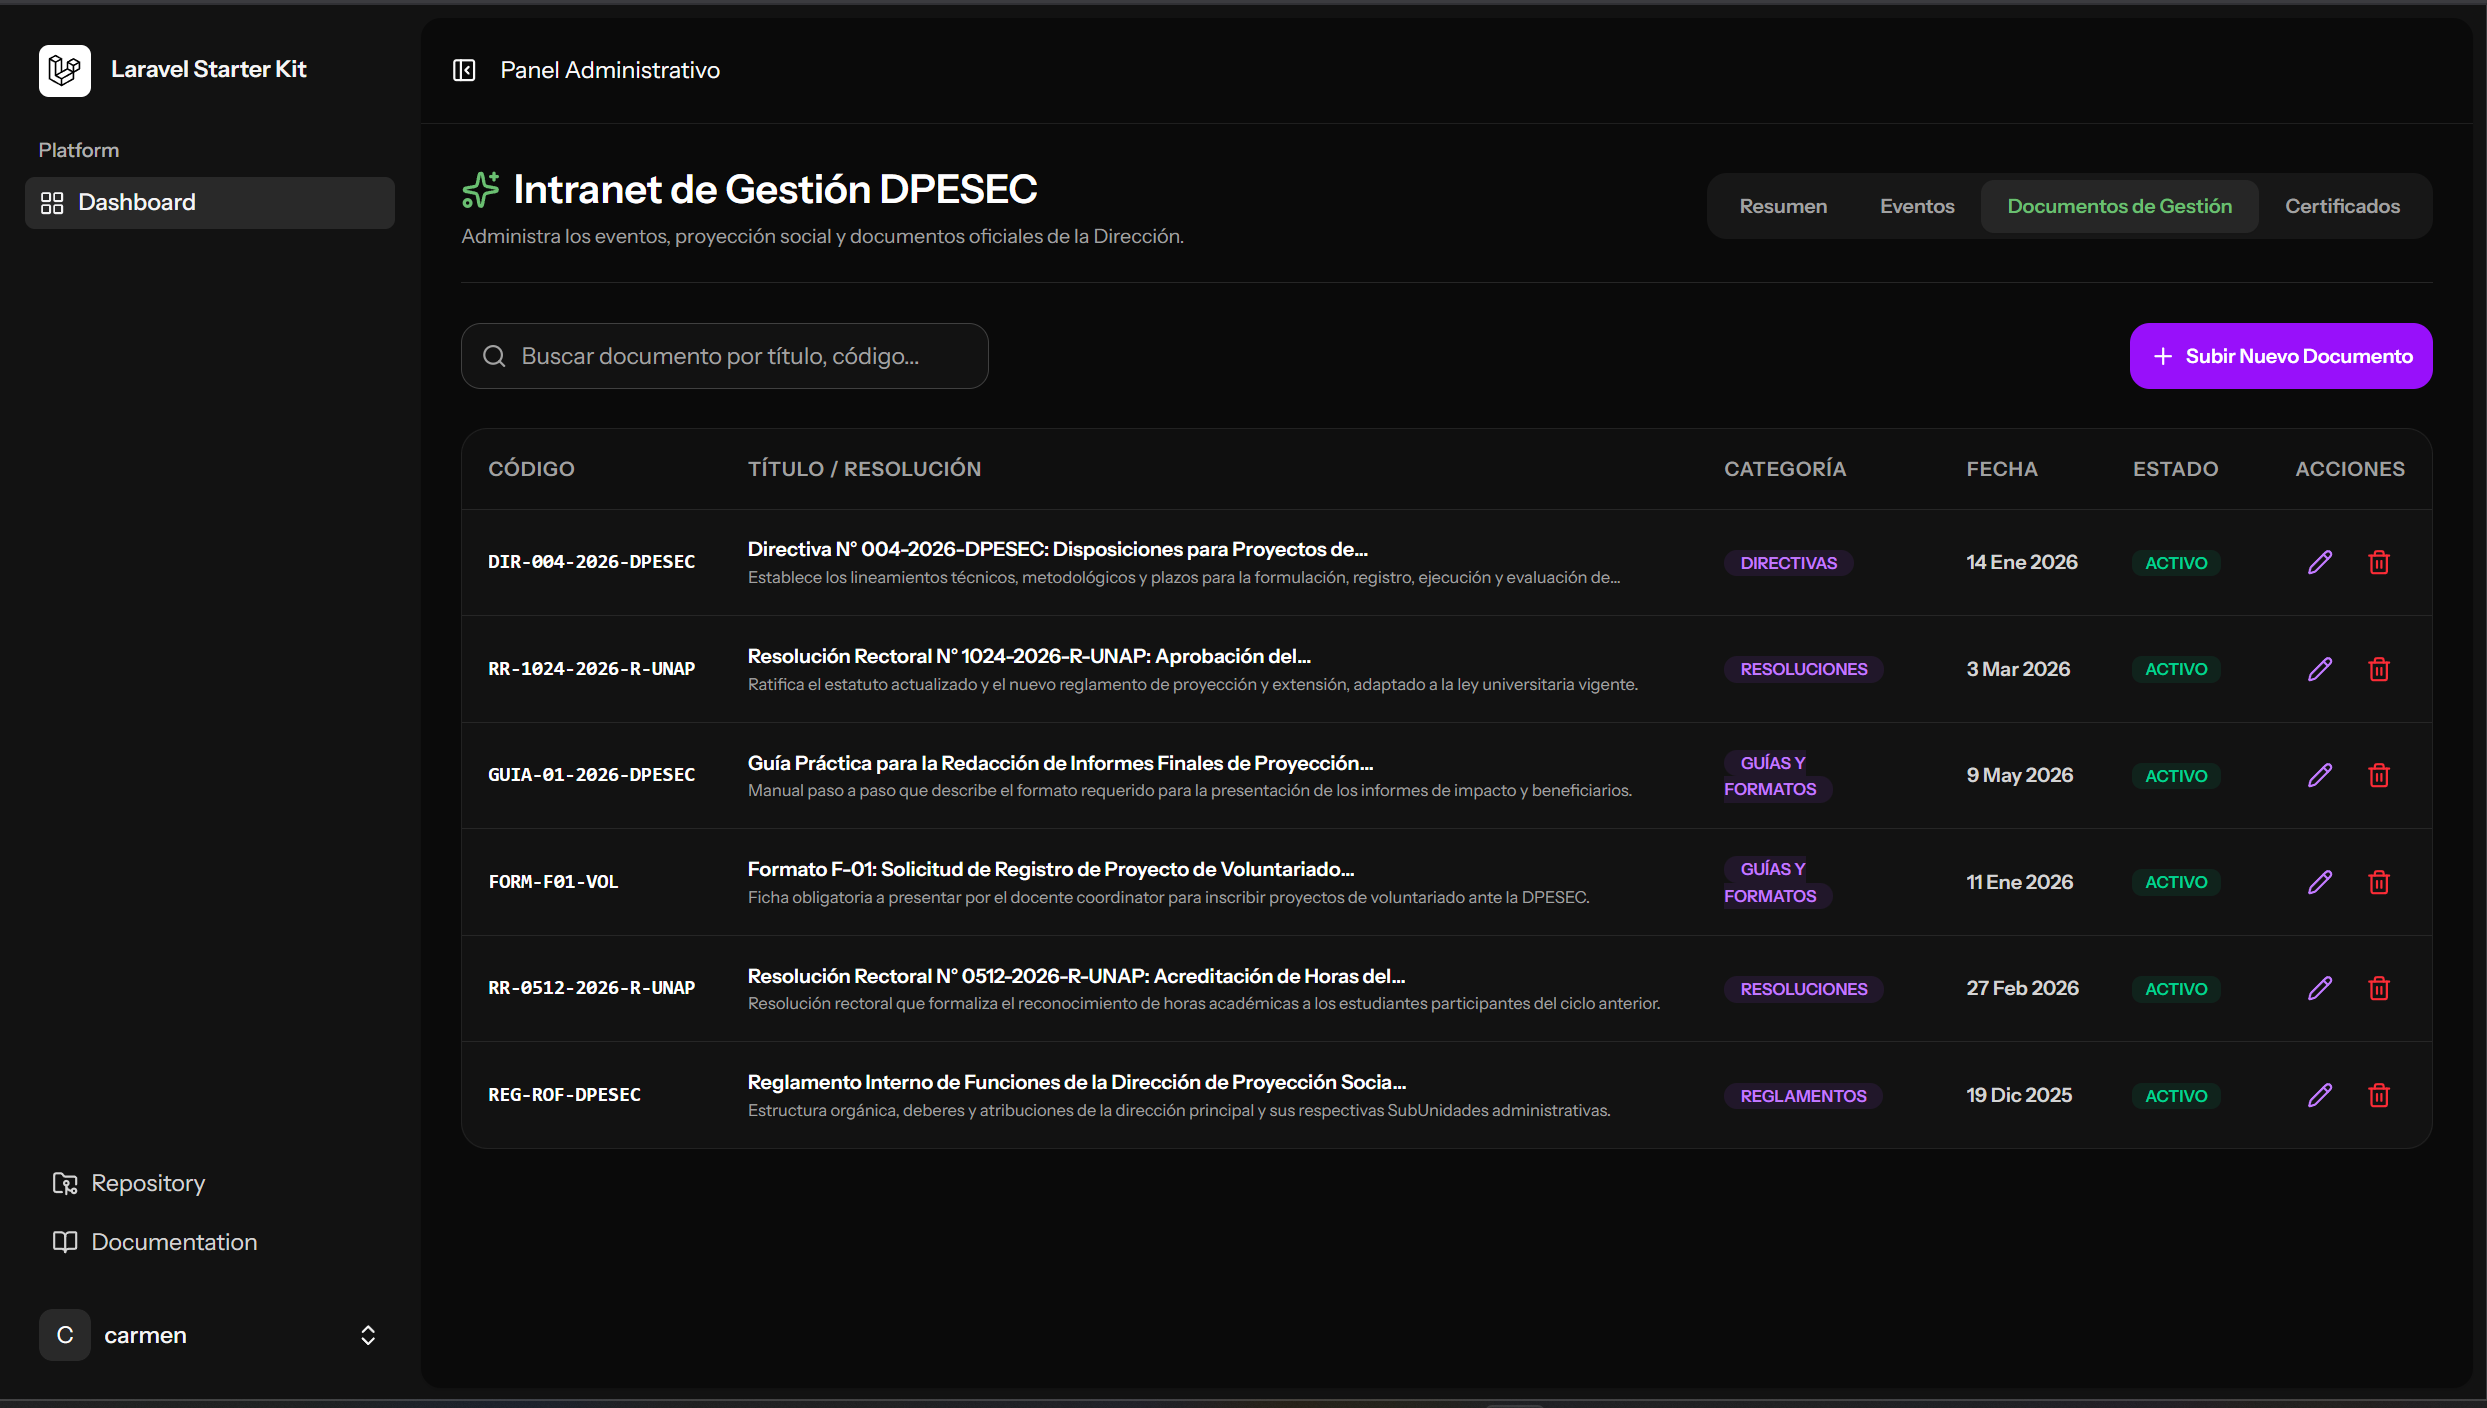
\includegraphics[width=0.8\textwidth]{img/dahsboard-intranet-documentosdegestion.png}
    \caption{Panel administrativo para la subida de directivas de gestión y normativas institucionales.}
\end{figure}

\begin{figure}[htbp]
    \centering
    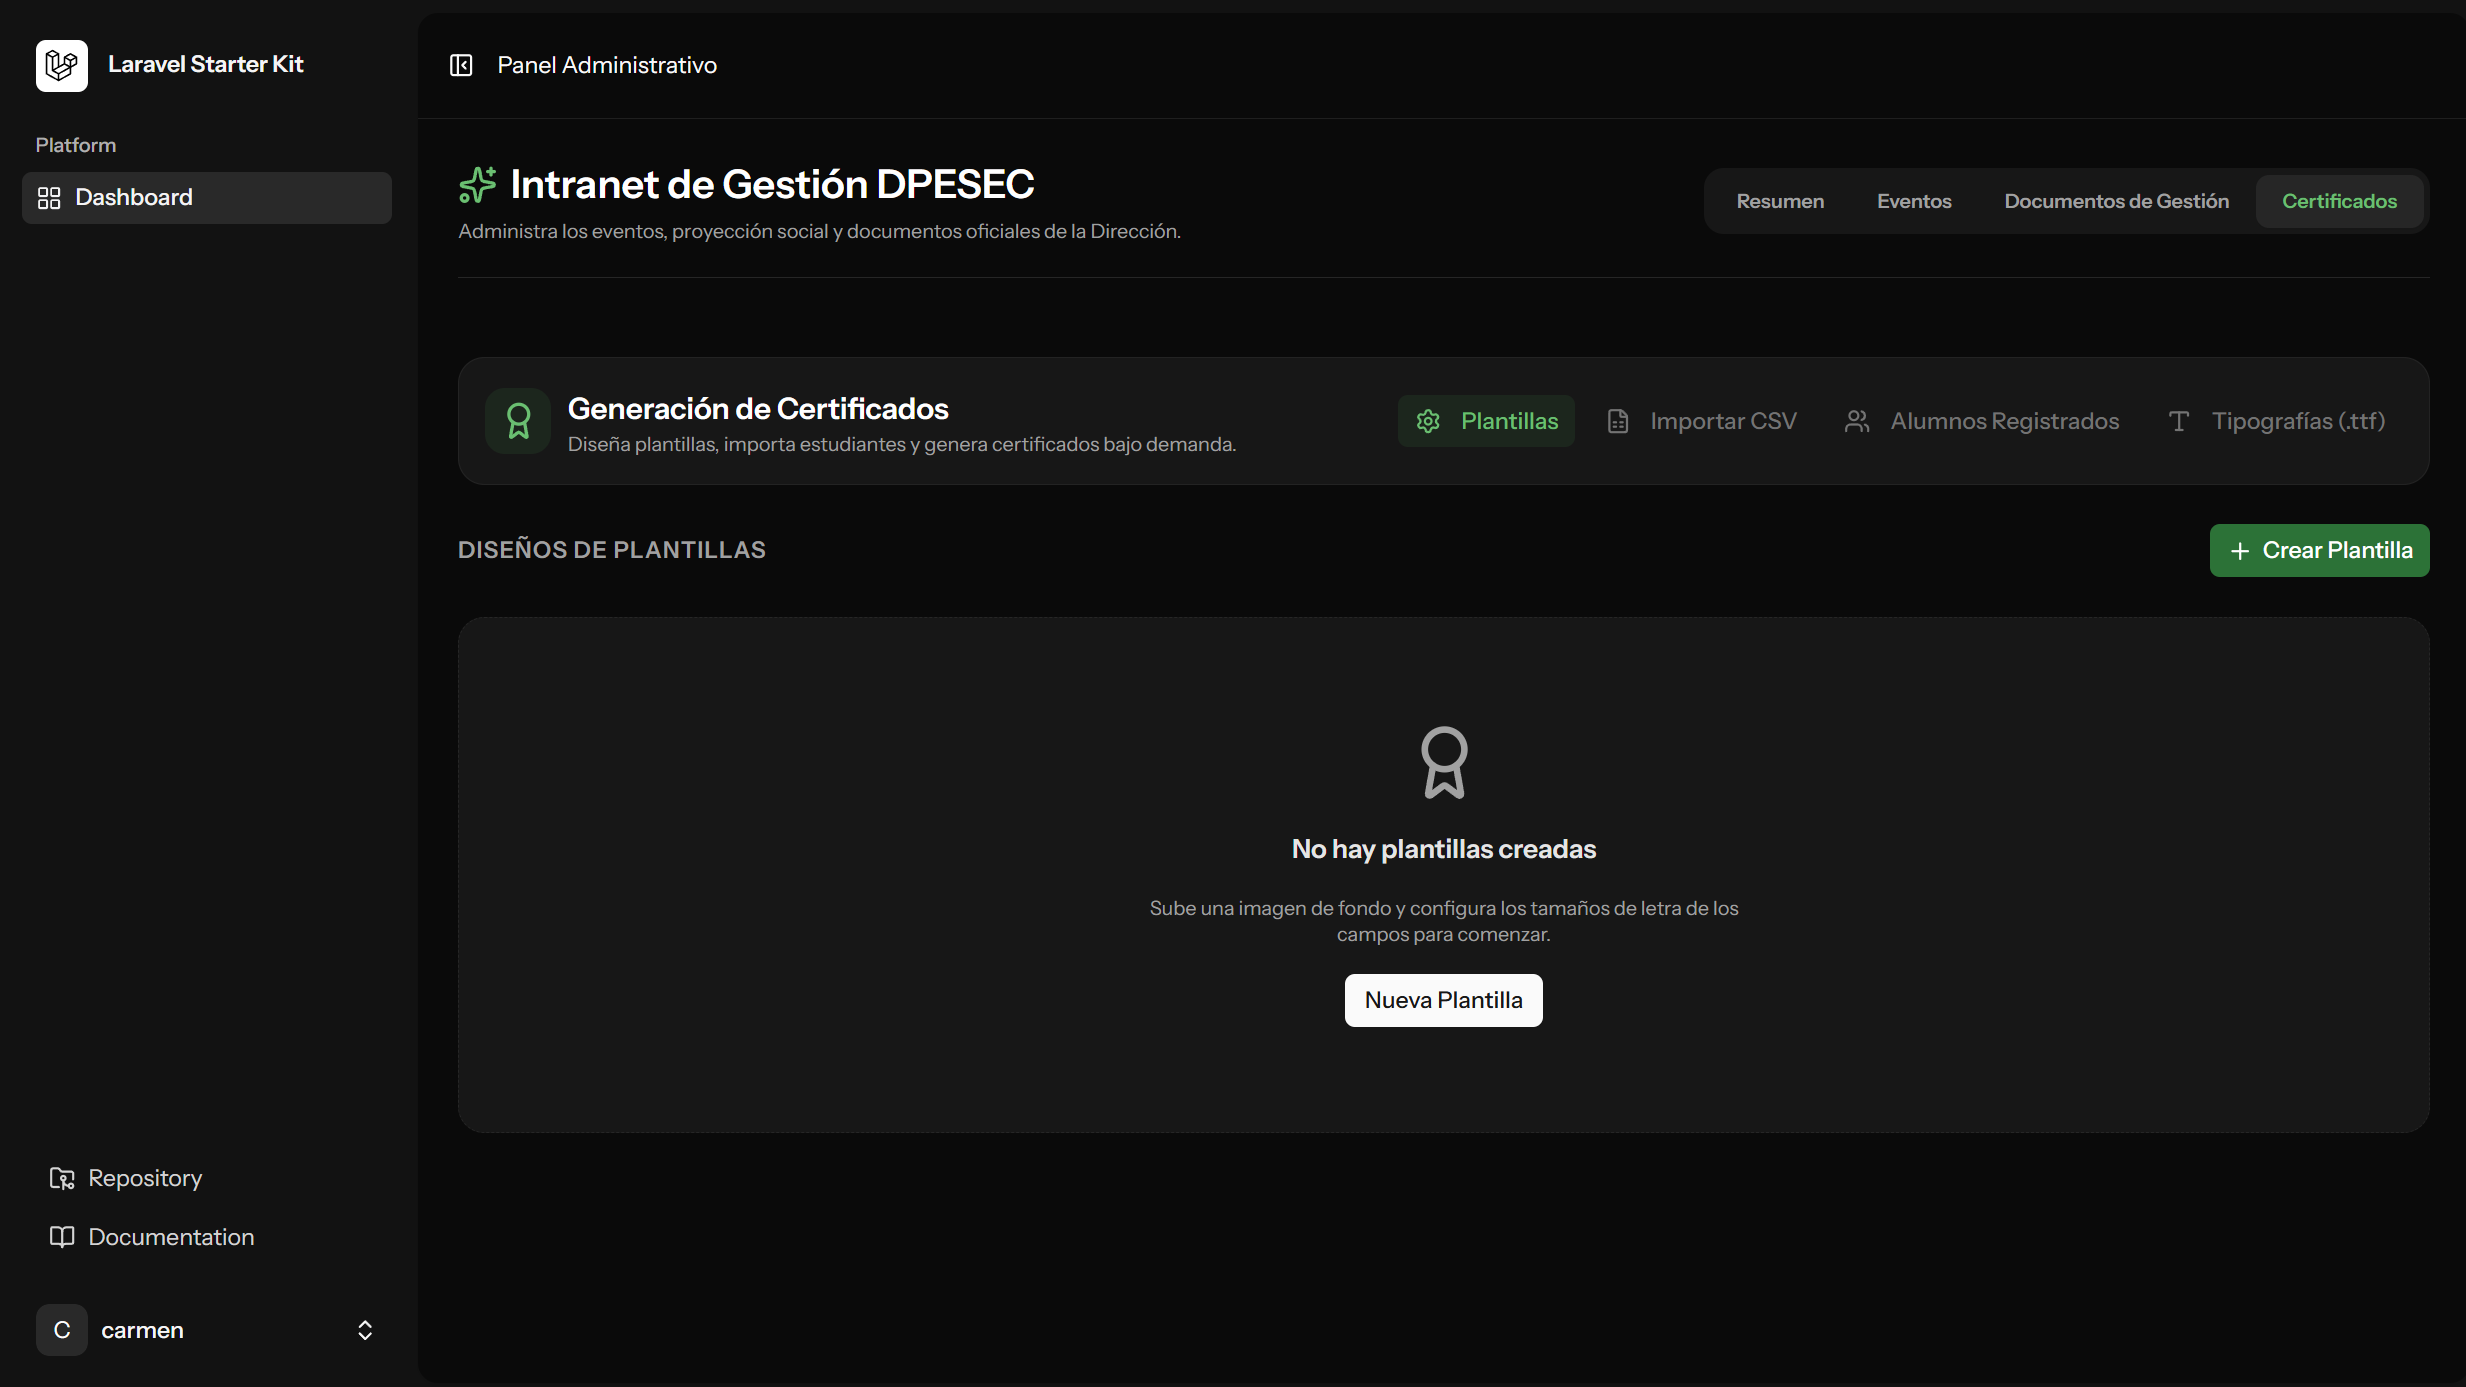
\includegraphics[width=0.8\textwidth]{img/dashboard-intranet-certificados.png}
    \caption{Gestor administrativo de certificados, plantillas base y subida masiva de participantes por CSV.}
\end{figure}

\begin{figure}[htbp]
    \centering
    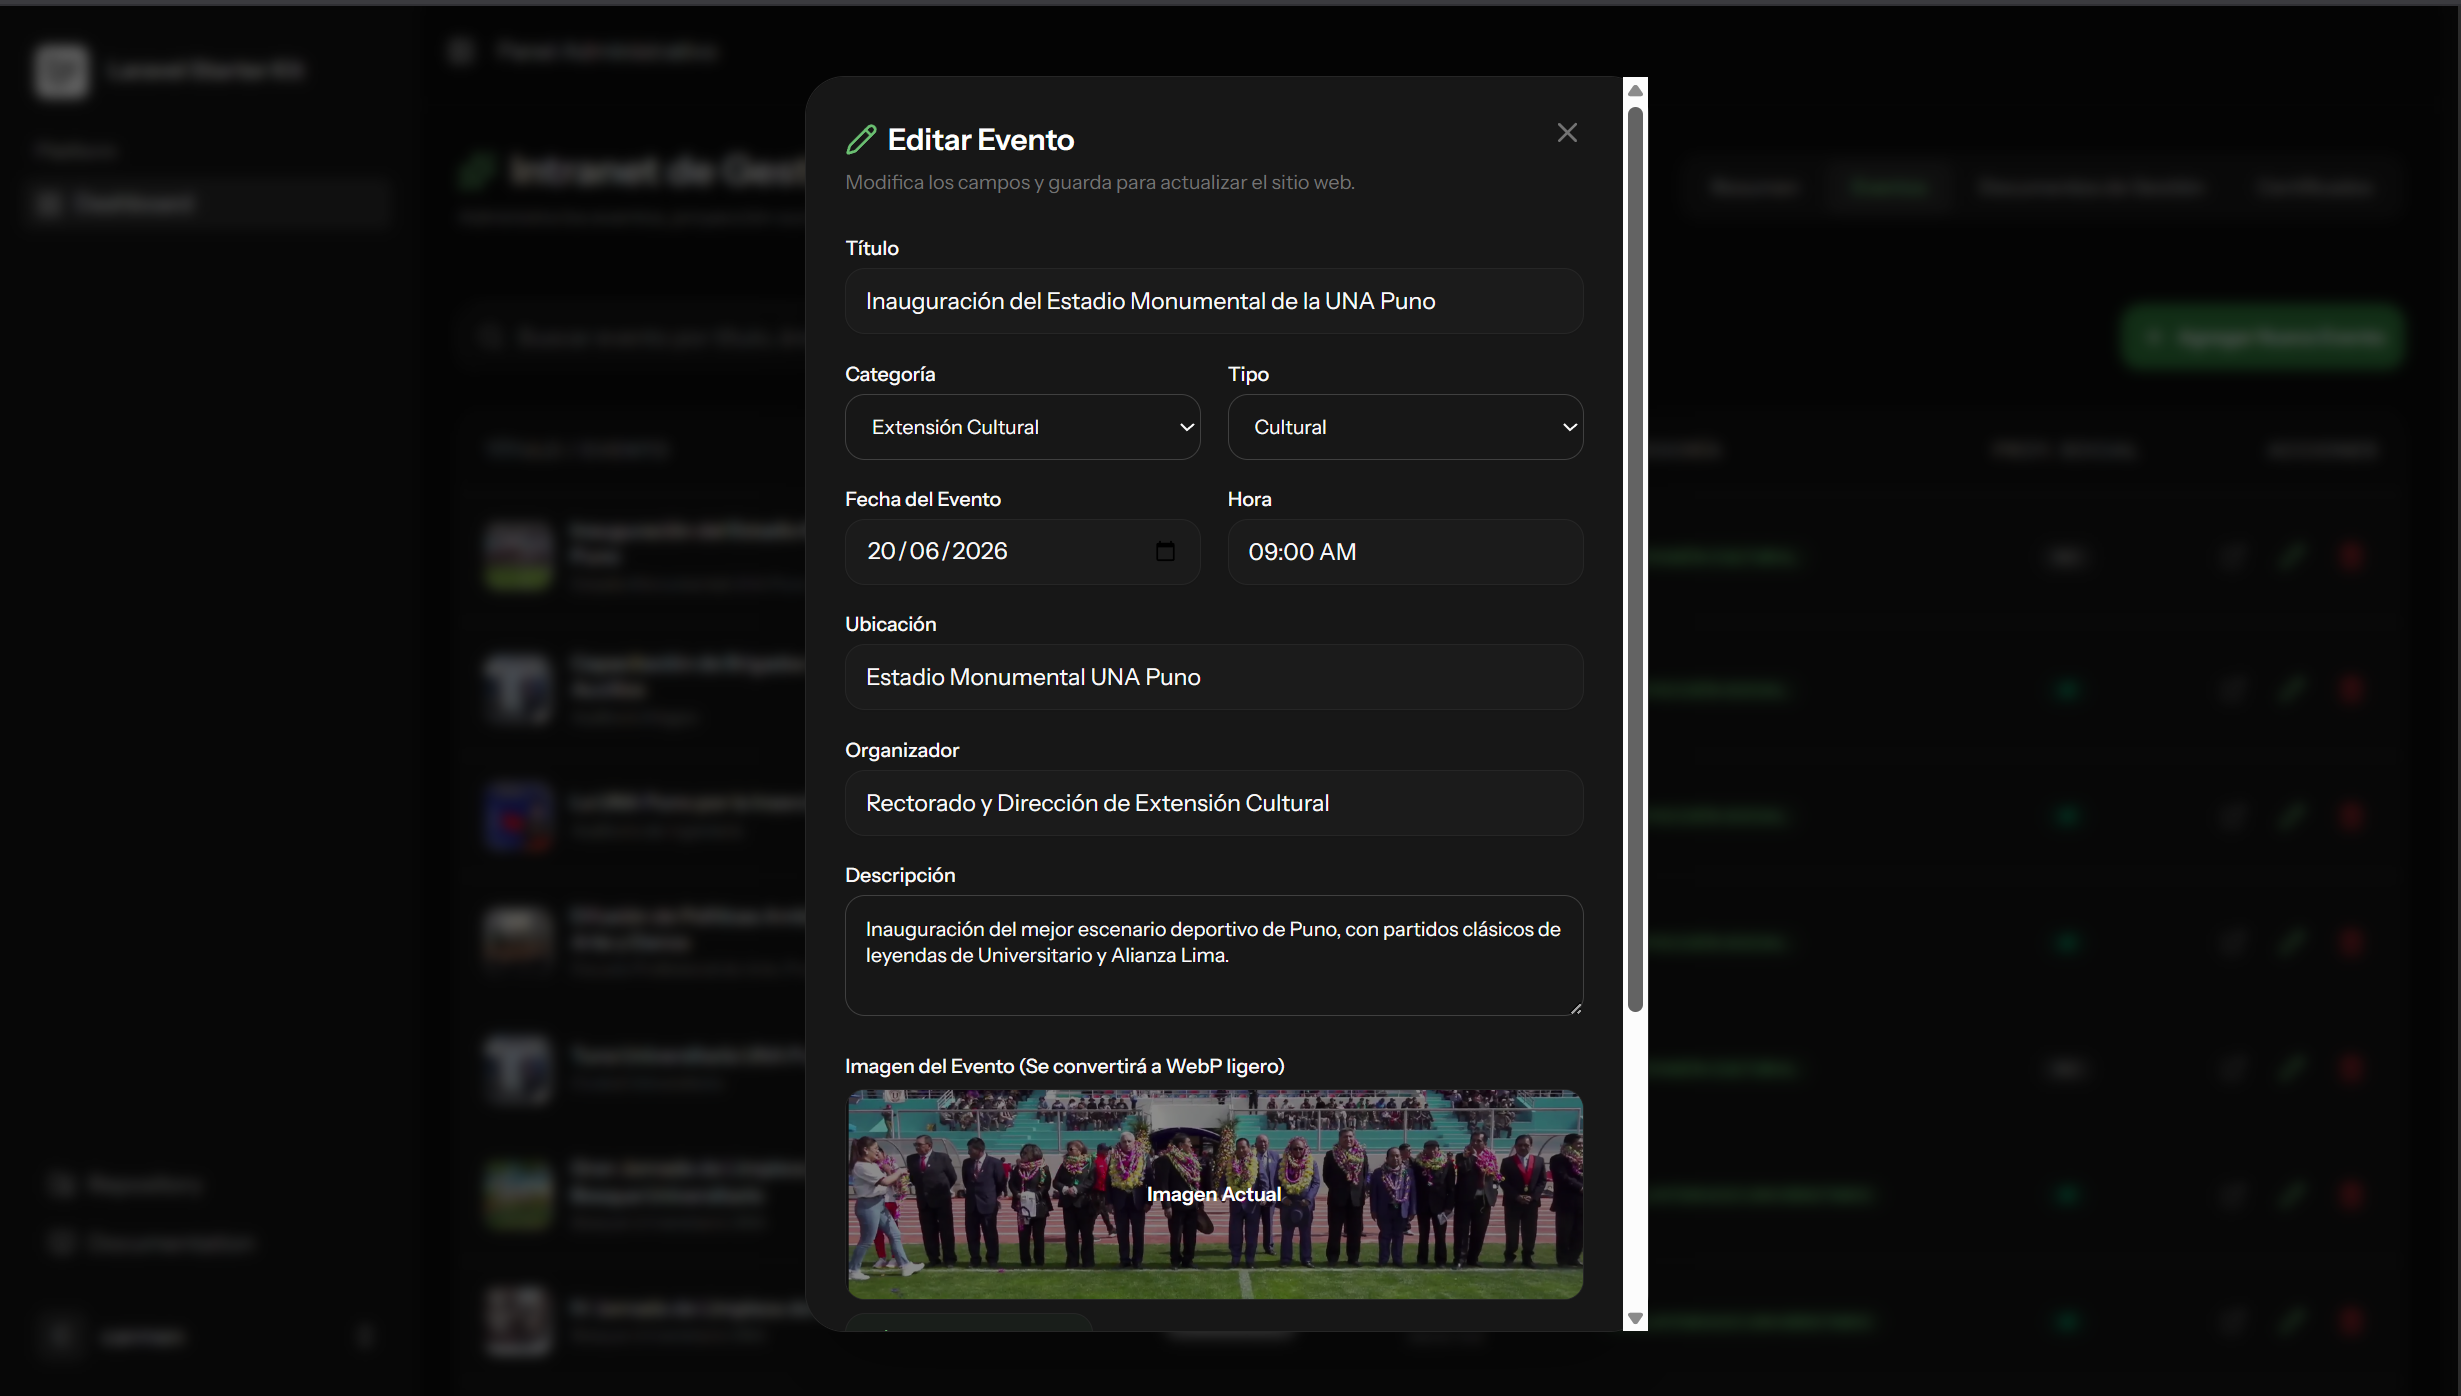
\includegraphics[width=0.8\textwidth]{img/dashboard-inttranet-editar_un_evento.png}
    \caption{Formulario interactivo de edición de evento con visor Canvas para mover, zoom y compresión a WebP.}
\end{figure}

\newpage

\subsection*{8.1. Fotografías de Actividades de Proyección Social}
Evidencias fotográficas de las campañas organizadas por la Dirección de Proyección Social y Extensión Cultural cuyas actas y participantes son gestionados por el sistema desarrollado.

\begin{figure}[htbp]
    \centering
    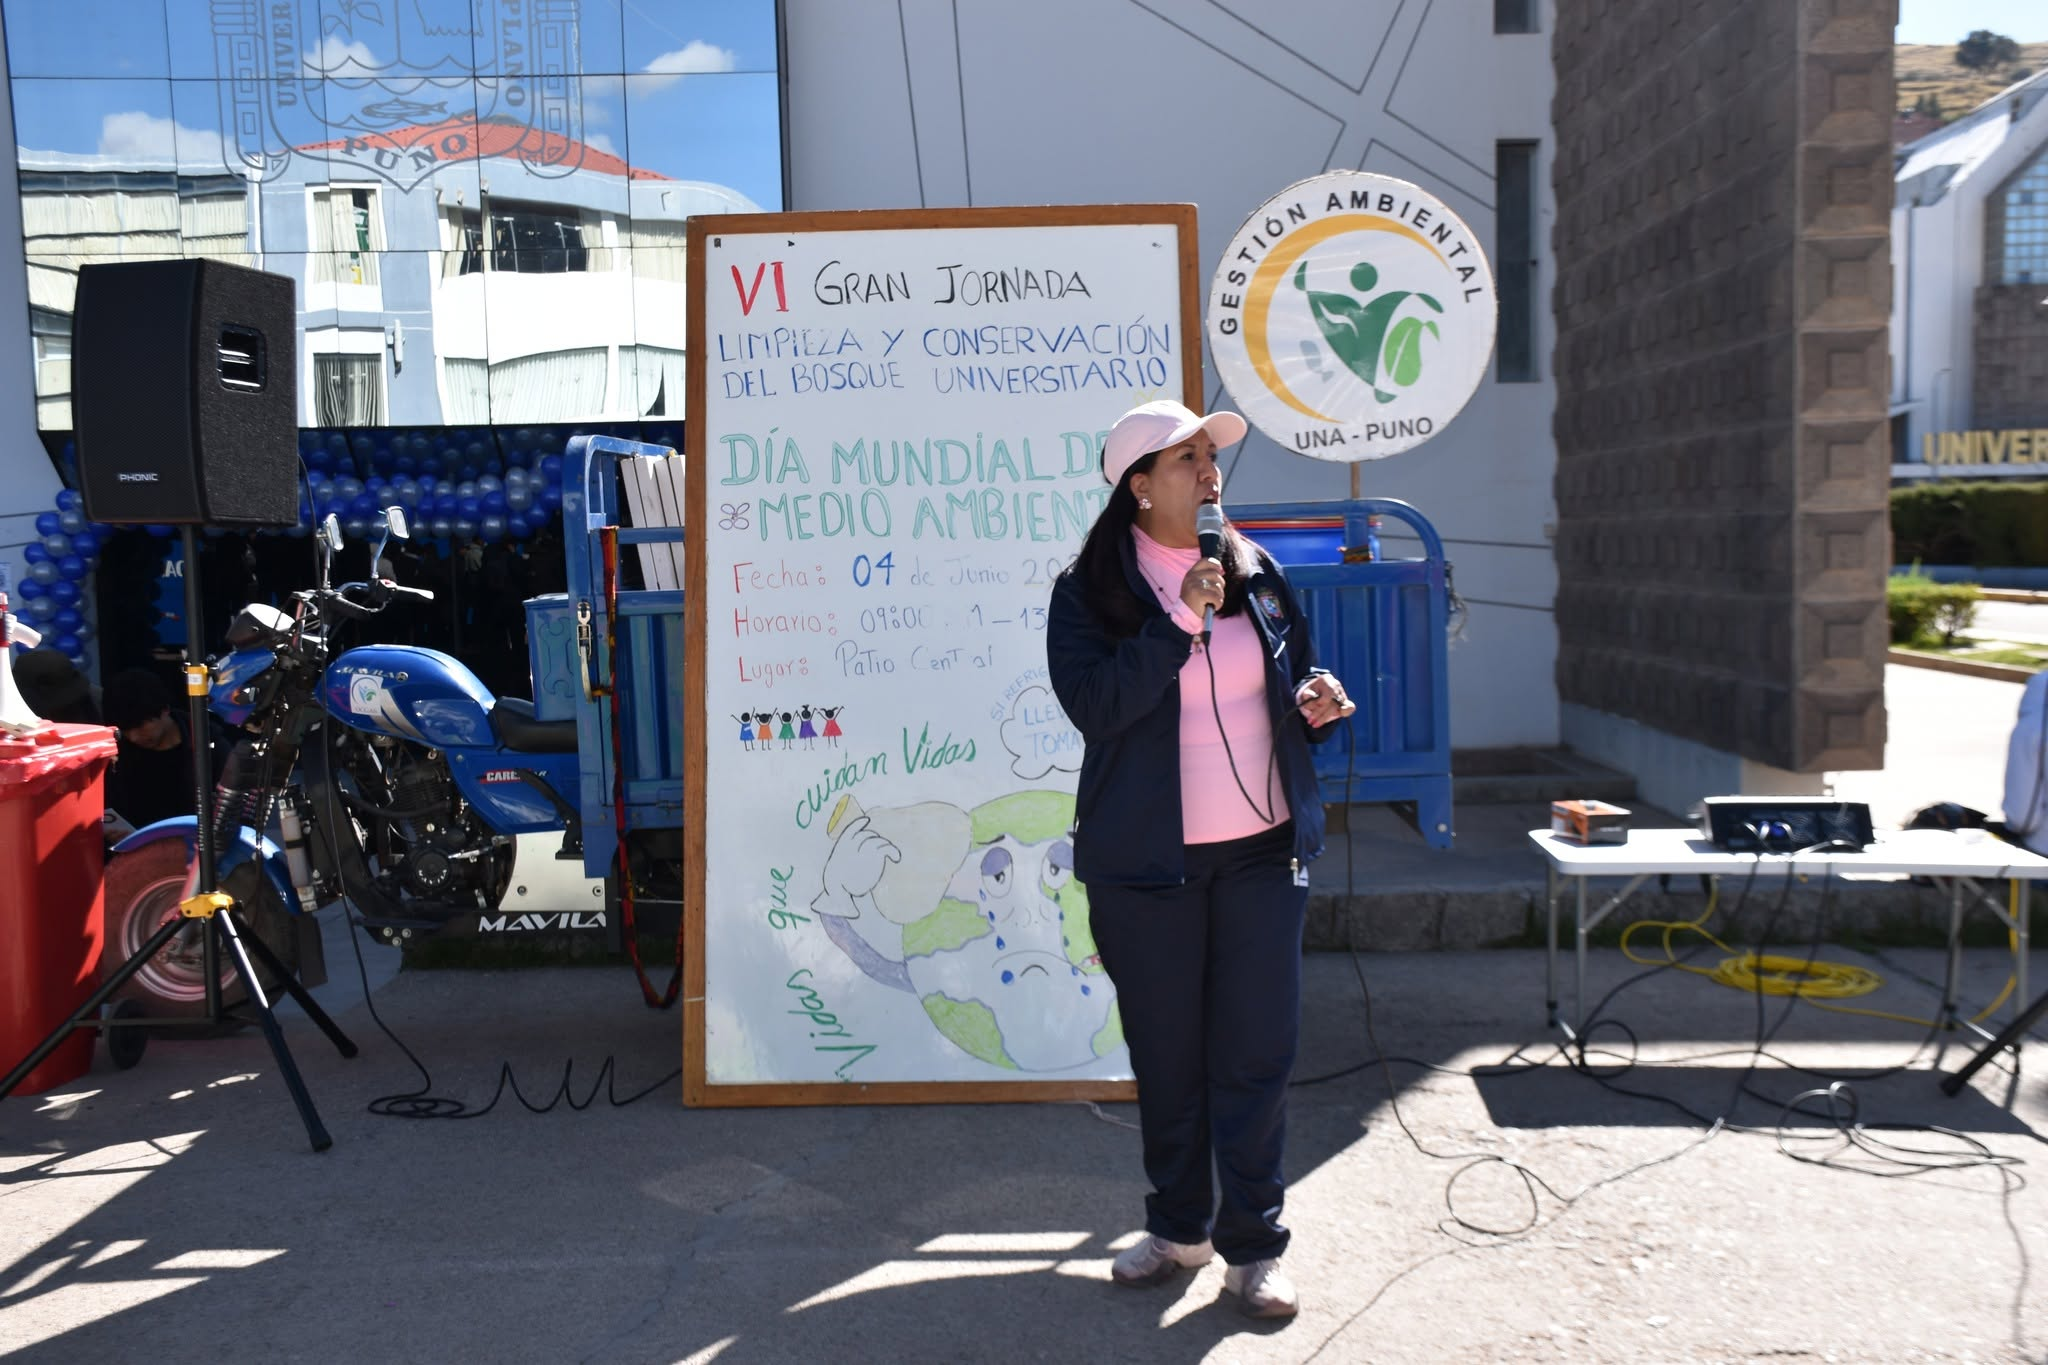
\includegraphics[width=0.7\textwidth]{img/brigadas_ambientales.jpg}
    \caption{Jornada de capacitación para las Brigadas Ambientales y Primeros Auxilios.}
\end{figure}

\begin{figure}[htbp]
    \centering
    
\includegraphics[width=0.7\textwidth]{img/gran_jornada.jpg}
    \caption{Gran Jornada de Limpieza y Conservación del Bosque Universitario de la UNA Puno.}
\end{figure}

\begin{figure}[htbp]
    \centering
    
\includegraphics[width=0.7\textwidth]{img/grabando_voces.jpg}
    \caption{Campaña de registro cultural "Grabando Voces del Quechua de Puno".}
\end{figure}

\begin{figure}[htbp]
    \centering
    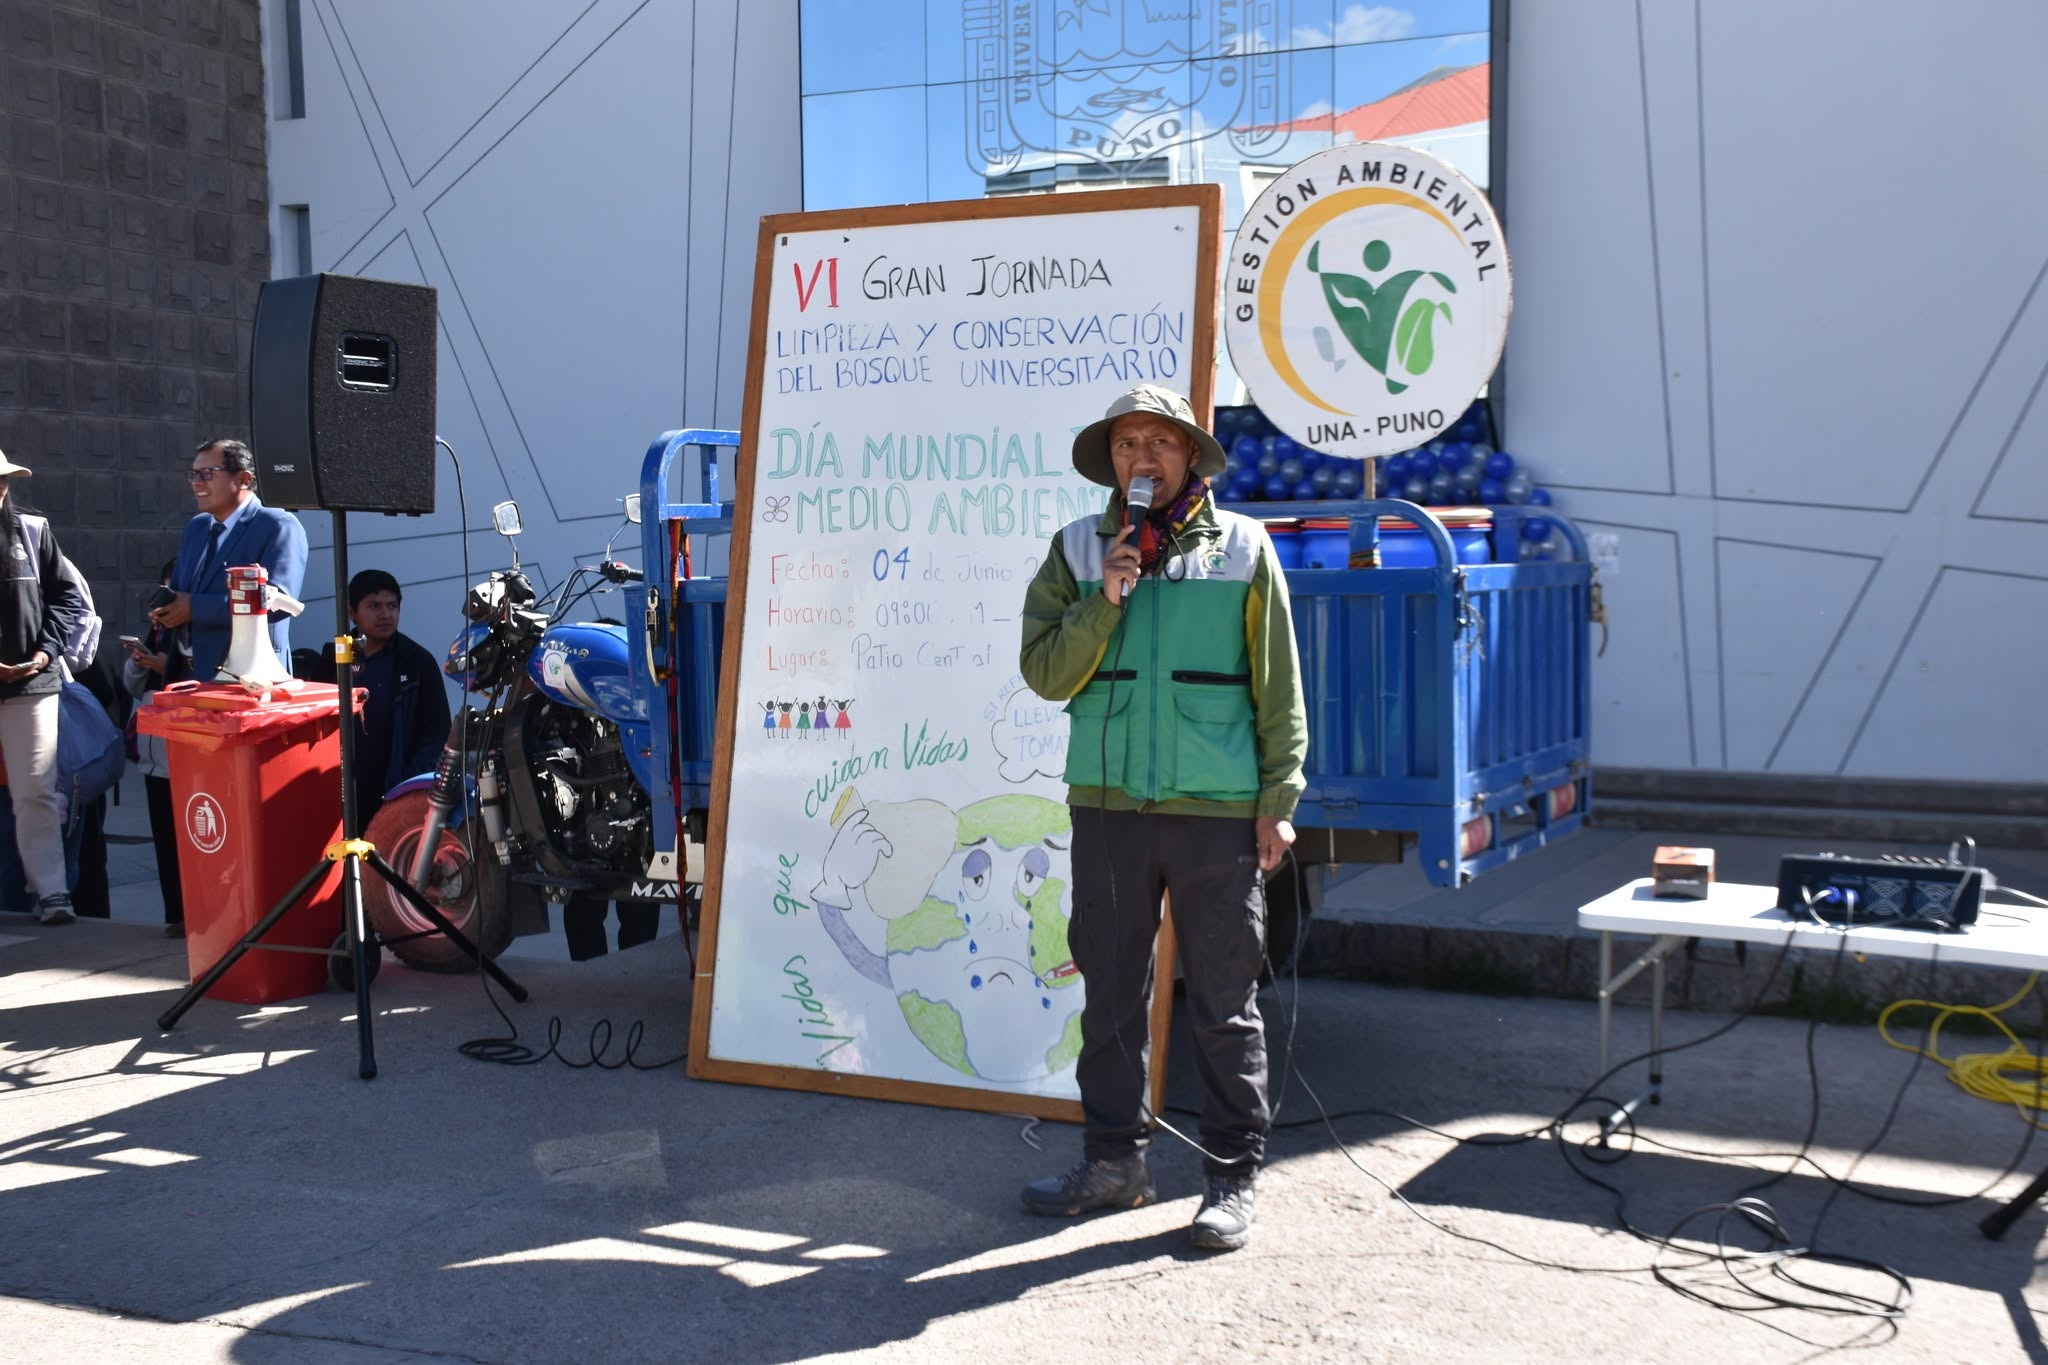
\includegraphics[width=0.7\textwidth]{img/limpieza_bosque.jpg}
    \caption{V Jornada de limpieza y reforestación participativa.}
\end{figure}

\begin{figure}[htbp]
    \centering
    
\includegraphics[width=0.7\textwidth]{img/insercion_laboral.jpg}
    \caption{Campaña de difusión para la inserción laboral y seguimiento de graduados.}
\end{figure}

\vspace{2cm}
\noindent
\begin{tabular}{c @{\hspace{3cm}} c}
    \rule{6.5cm}{0.5pt} & \rule{6.5cm}{0.5pt} \\
    \textbf{Jefe Inmediato del Centro de Prácticas} & \textbf{Docente Supervisor} \\
    DRA. MILDER ZANABRIA ORTEGA & M.Sc. WILDO SUCASAIRE MONROY \\
    Director de la DPSEC & Escuela Profesional de Ingeniería de Sistemas \\
\end{tabular}

\end{document}
